%% TO DO:
%% TITOLO CAP 6
%% TABLE OF CONTENTS
%% BIBLIOGRAPHY STYLE
%% GRAFICO CONVERGENCE DT hartris

\documentclass[krantz2,a4paper,11pt,ChapterTOCs,twoside,openright]{krantz}
%\usepackage{fixltx2e,fix-cm}
\usepackage[utf8]{inputenc}
\usepackage[english]{babel}
\usepackage{csquotes}
%\usepackage{lmodern}  % allows flexible font sizes
\usepackage{amssymb}
\usepackage{amsmath}
\usepackage{amsthm}
\usepackage{graphicx}
\usepackage{subfigure}
%\usepackage{makeidx}
\usepackage[bottom]{footmisc} % places footnotes at page bottom
\usepackage{bm}
%\usepackage{multicol}
%\usepackage{textgreek}
%\usepackage[normalem]{ulem}	  % for strike-through of text with \sout{}

%% PAGE LAYOUT
%\usepackage{showframe}
%\widowpenalty=300  % penalties for widow lines
%\clubpenalty=300
\frenchspacing
\tolerance=5000

%% TABLES
%\usepackage{longtable}
%\usepackage{booktabs}
\usepackage{array}
\renewcommand{\arraystretch}{1.2}

%% FIGURES
\usepackage[section]{placeins}  % place floats within section
\usepackage[]{caption}
%\usepackage[labelfont={small,bf},textfont=small]{caption}
\renewcommand{\captionfont}{\fontsize{10}{12}\selectfont}
\renewcommand{\captionlabelfont}{\bfseries\fontsize{10}{12}\selectfont}
\captionsetup{width=0.9\textwidth}
%\usepackage{subcaption}

%% BIBLIOGRAPHY
%\usepackage[numbers,sort&compress]{natbib}

\usepackage[backend=biber,style=phys,sorting=none,hyperref=true,articletitle=true,doi=true,biblabel=brackets,chaptertitle=true,pageranges=false]{biblatex}
%\renewcommand{\bibfont}{\small}  % customized bibliography style
%\setlength{\bibitemsep}{5pt}
\newcommand{\printpublication}[1]{\AtNextCite{\defcounter{maxnames}{99}}\fullcite{#1}}
\addbibresource{bibliography.bib}


%% PDF STUFF
\usepackage{url}
%\usepackage{colortbl}
\usepackage{hyperref}
%\usepackage[inner,right]{showlabels}

%% EDITOR COMMANDS
%\usepackage[usenames,dvipsnames]{color}
%\newcommand{\editor}[2]{%
%  \expandafter\newcommand\csname #1note\endcsname[1]{%
%    \textcolor{#2}{(\textbf{#1:} \emph{\textsf{##1}})}}%
%  \expandafter\newcommand\csname #1\endcsname[1]{%
%    \textcolor{#2}{##1}}%
%  \expandafter\newcommand\csname #1cancel\endcsname[1]{%
%    \textcolor{#2}{\sout{##1}}}%
%  \expandafter\newcommand\csname #1change\endcsname[2]{%
%    \textcolor{#2}{\sout{##1} ##2}}%
%  \newenvironment{#1text}{\color{#2}}{\color{black}}
%}
%\definecolor{blue}{rgb}{0,0.4,0.7}
%\definecolor{tangerine}{rgb}{0.944,0.522,0}
%\definecolor{verde}{rgb}{0,0.5,0}
%\editor{LE}{blue}
%\editor{SB}{tangerine}

%% TABLE OF CONTENTS
%\makeindex
\setcounter{tocdepth}{2}

%% DEFINITIONS
\newtheorem{theorem}{Theorem}
\newtheorem{lemma}{Lemma}
\DeclareMathAlphabet\mathbfcal{OMS}{cmsy}{b}{n}  % bold mathcal letters
\newcommand{\hbindex}[1]{\hl{#1}\index{#1}}  %highlights index entries
\def\smallgamma{{\scriptscriptstyle \gamma}}
\def\smallone{{\scriptscriptstyle 1}}
\def\smallE{{\scriptscriptstyle E}}
\def\smallQ{{\scriptscriptstyle Q}}
\def\smallZ{{\scriptscriptstyle Z}}
\def\smallXC{{\scriptscriptstyle XC}}
\def\smallDFT{{\scriptscriptstyle DFT}}
\def\smallGGA{{\scriptscriptstyle GGA}}
\def\smallH{{\scriptscriptstyle H}}
\def\smallKS{{\scriptscriptstyle KS}}
%\def\eqref#1{(\ref{#1})}
\def\angstrom{{\mbox{\AA}}}
\def\S1{{\mathbb{S}_1}}
\newcommand{\un}[1]{\,\mathrm{#1}}
%\newcommand{\red}[1]{\textcolor{red}{#1}}
\def\rGamma{{\mathrm\Gamma}}
\def\rDelta{{\mathrm\Delta}}
\def\rLambda{{\mathrm\Lambda}}
\def\rOmega{{\mathrm\Omega}}
\def\abinitio{\emph{ab initio} }

%%%%%%%%%%%%%%%%%%%%%%%%%%%%%%%%%%%%%%%%%%%%%%%%%%%%%%%%%%%%%%%%%%%%%%%%%%
\begin{document}

\frontmatter
\title{ab initio simulation of heat transport in silica glass}
\author{Loris Ercole}
%\maketitle
\begin{titlepage}
\begin{center}

  \voffset 1. cm
\textsc{\Large Scuola Internazionale Superiore di Studi Avanzati} %[0.5cm]
\vskip 0.75cm
\hrule height 1 pt
\vskip 0.75cm
\textsc{\fontsize{14}{16}\selectfont PhD course in Theory and Numerical Simulation\\
of Condensed Matter}
\vskip 0.5cm

 \begin{figure}[h]
 \centering
 \includegraphics[width=5.5cm]{frontmatter/SISSA_40_alt.png}
 \end{figure}

\vskip 0.5 cm
\hrule height 1 pt
\vskip 1.6 cm
%%%Title
% { \Huge \bfseries  Aspetti di Meccanica Quantistica Supersimmetrica}\\[0.4cm]
{ \fontsize{20}{22} \bfseries  \emph{ab initio} Simulation of Heat Transport \\
\vspace{0.4cm}
in Silica Glass
}
\vfill

%\vskip 5.4 cm
{A thesis submitted for the degree of \textit{Doctor Philosophiae}}
\vskip 1.5 cm

\begin{center}
\begin{minipage}{0.3\textwidth}
\fontsize{12}{14}\selectfont
\emph{Supervisor}\\
\smallskip
Prof.~Stefano \textsc{Baroni}
\end{minipage}
\hspace{2cm}
\begin{minipage}{0.3\textwidth}
\fontsize{12}{14}\selectfont
\emph{Candidate}\\
\smallskip
Loris \textsc{Ercole}
\end{minipage}
\end{center}
\vspace{1cm}

%\begin{flushleft} \normalsize
%\emph{Supervisor}\\
%Prof. ~Stefano  \textsc{Baroni}
%\end{flushleft}

%\vspace{-42 pt}
%\hspace{9.6cm}
%\begin{minipage}{4.2cm}
    %%% \vskip 2.cm
%    \begin{flushleft} \normalsize
%    \end{flushleft}
%\end{minipage}
%%%% \vskip 1.595 cm

\hrule height 1.1 pt
\vskip 0.5cm

\textsc{\large October 2018}

\end{center}

\end{titlepage} 
\cleardoublepage
\thispagestyle{empty}
\vspace*{\stretch{1}}
\begin{flushright}
\Large\itshape
To my parents.
\end{flushright}
\vspace{\stretch{3}}
\cleardoublepage
\chapter*{Ringraziamenti}

Ricordo ancora, meno di quattro anni fa, il momento in cui iniziai ad avventurarmi in questo misterioso universo del trasporto termico. Mai avrei immaginato che in pochi anni questo progetto si sarebbe sviluppato e ramificato in così tanti e variegati aspetti, sia pratici, rivelatisi tutt'altro che banali e scontati, sia fondamentali, con inaspettati fondamenti teorici che stanno tutt'ora venendo a galla e che non smettono di affascinarmi. 
Senza dubbio, tutto questo percorso di ricerca non sarebbe stato possibile senza la guida e il sostegno del mio supervisor, Stefano Baroni, a cui va la mia profonda stima e gratitudine. È grazie a lui se mi sono appassionato a questo tema e alla ricerca. 

Devo un grosso ringraziamento anche ad Aris Marcolongo, con cui ho collaborato in molti aspetti di questo lavoro, e a Federico Grasselli e Riccardo Bertossa, con cui ho condiviso gli ultimi due anni del mio soggiorno alla SISSA, per le innumerevoli discussioni in macchina tra Trieste e Verona, e per l'aiuto e l'ispirazione in molteplici problemi.

Quattro anni a Trieste sono passati in un lampo, e questo lo devo interamente a tutti gli amici che hanno condiviso con me questo viaggio, chi prima o chi dopo, sono riconoscente a tutti voi: 
Mariami, Maja, Leyla, Sara, Federico, Riccardo, Ivan, Luca, Francesco, Simone, Tommaso, Caterina, Seher, Nina, Matteo, Juraj, Mattia, Stefano, Tommaso, Francesco, Nicolò, Lorenzo, Federico, Marco, e molti altri.

Nondimeno, devo ringraziare tutti gli amici di Verona, che pur vedendo sporadicamente, mi fanno sempre sentire a casa: i miei compagni Agorà, con cui abbiamo raggiunto traguardi incredibili (e spero sia solo l'inizio!), gli amici di mille più imprevedibili avventure, e gli amici storici su cui puoi sempre contare e che ho sempre il piacere di rincontrare. 

Infine, il ringraziamento più grande va alla mia famiglia e in particolare ai miei genitori, a cui dedico questo lavoro, e senza i quali non avrei davvero potuto raggiungere questo traguardo. \textbf{GRAZIE!}

\cleardoublepage
%\setcounter{page}{7} %previous pages will be reserved for frontmatter to be added in later.

\tableofcontents
% \include{frontmatter/symbollist}

\mainmatter
\thischaptertocfalse
\chapter{Introduction}

Ciao sticazzi

\section{AAIAIIA}

fff  % Introduction
\thischaptertoctrue
\chapter{Green-Kubo theory of heat transport}  \label{ch:green-kubo}

Our microscopic understanding of heat and mass transport in extended systems is rooted in the Green-Kubo (GK) theory of linear response,\cite{Green1954,Kubo1957a} as applied to the Navier-Stokes equations for the densities of the conserved extensive variables,\cite{Kadanoff1963,Forster1975} which include energy, momentum, and the particle numbers for each molecular species. 
\begin{LEtext}
The fluctuation-dissipation theorem establishes a relation between the (non-equilibrium) transport coefficients and the spontaneous fluctuations of the relevant currents at equilibrium. Transport coefficients are in fact proportional their the autocorrelation times.

In this chapter we briefly walk through the theory that allows the derivation of the Green-Kubo equations for transport coefficients, starting from the definition of the hydrodynamic variables of a system, and the use of the linear response theory to connect equilibrium properties to non-equilibrium ones. We then specialize to the case of heat transport in solids and one component fluids, and the particular case of multi-component fluids, and we derivee the expression of the energy flux for systems described by classical force fields.
\end{LEtext}


\section{Hydrodynamic variables} \label{sec:hydrodyn_var}
The macroscopic processes occurring in condensed matter are often described in terms of \emph{extensive variables}. By definition, the value that such a variable assumes for a system is the sum of the values it has for each of its subsystems. This property allows one to express an extensive variable, $A$, as the integral of a suitably defined density, $a(\mathbf{r})$, as:
\begin{equation}
A[\rOmega]=\int_\rOmega a(\mathbf{r})d\mathbf{r}, \label{eq:extensivity}
\end{equation}
where $\rOmega$ is the system volume. Here and in the following boldfaces indicate 3D vectors and Greek subscripts label Cartesian components: $\mathbf{u}= \{u_\alpha\} = \{u_1,u_2,u_3\}$. When an extensive quantity is locally conserved, a current density, $\bm{j}(\mathbf{r},t)$, can be associated to its density in such a way that the two of them satisfy the continuity equation:
\begin{equation}
\frac{\partial a(\mathbf{r},t)}{\partial t} = - \nabla\cdot\bm{j}(\mathbf{r},t), \label{eq:continuity}
\end{equation}
where $\nabla\cdot\bm{j}$ indicates partial differentiation and the middle dot a scalar product (a divergence in this case). In the following the densities and current densities of conserved quantities will be called \emph{conserved densities} and \emph{conserved currents} for short. The space Fourier transform of Eq.~\eqref{eq:continuity} reads:
\begin{equation}
\dot{\tilde a}(\mathbf{q},t) = - i\mathbf{q} \cdot \tilde {\bm{\jmath}} (\mathbf{q},t), \label{eq:kontinuity}\end{equation}
where the overdot indicates a time derivative and the tilde a Fourier transform, so that the longer the wavelength, the slower is the dynamics of a conserved density. We conclude that for long enough wavelengths, conserved densities are adiabatically decoupled from all the other (zillions of) fast atomic degrees of freedom. Note that in this chapter we are using the concept of \emph{adiabatic decoupling} in two distinct senses, depending on the context: to indicate the decoupling of electronic from nuclear degrees of freedom, and that of hydrodynamic variables from fast atomic ones.

The long-wavelength Fourier components of conserved densities are called \emph{hydrodynamic variables}. In macroscopically homogeneous systems, different wavelengths are decoupled from each other, while, as we have seen, the long wavelengths are adiabatically decoupled from all the other degrees of freedom. Let us suppose there are $Q$ conserved extensive variables. In the case of a mono-atomic fluid, for instance, $Q=5$, corresponding to mass (or particle number), energy, and the three components of the momentum. In order to simplify the notation, we set the value of the conserved quantities equal to zero, $A^i=0$, so that their densities, $a^i(\mathbf{r})$, directly refer to the departure from equilibrium, and we indicate by $\bm j^i(\mathbf{r},t)$ the corresponding currents. At equilibrium, all the conserved densities and currents vanish. Off equilibrium, it will be assumed that the wavelength and the time scale of the disturbances are so long that thermal equilibrium still holds \emph{locally}. That is to say, a local temperature, pressure, and chemical potential can be defined, such that, when combined with the densities of extensive variable, they satisfy a local equation of state.

For small enough deviations from equilibrium, the time derivatives of conserved densities are linear combinations of the densities themselves. In the frequency/wavevector domains this condition can be expressed as
\begin{equation}
  -i\omega\tilde a^i(\mathbf{q},\omega) = \sum_j \tilde\rLambda^{ij}(\mathbf{q},\omega) \tilde a^j(\mathbf{q},\omega), \label{eq:Fourier-continuity}
\end{equation}
where the tilde indicates now a space-time Fourier transform: $\tilde a(\mathbf{q},\omega) = \int \mathrm{e}^{-i(\mathbf{q}\cdot \mathbf{r}-\omega t)} a(\mathbf{r},t)d\mathbf{r}dt $. By combining Eq.~\eqref{eq:Fourier-continuity} with the time Fourier transform of Eq.~\eqref{eq:kontinuity}, we obtain the so-called constitutive equations for the (longitudinal components of the) conserved currents:
\begin{equation}
  \tilde{\bm{\jmath}}^i(\mathbf{q},\omega)=i\frac{\mathbf{q}}{q^2} \sum_j\tilde \rLambda^{ij}(\mathbf{q},\omega)\tilde a^j(\mathbf{q},\omega). \label{eq:constitutive-qomega}
\end{equation}
In isotropic media, the $\tilde\rLambda$'s are spherically symmetric functions of $\mathbf{q}$, whereas their value at $\mathbf{q}=0$ vanishes, because a non-vanishing value would imply a non-physical long-range dependence of the currents on density fluctuations, in contrast with our assumption of local thermodynamic equilibrium. The long-wavelength low-frequency limit of the coupling constants can thus be assumed to be $\tilde\rLambda^{ij}(\mathbf{q},\omega) \sim q^2 \lambda^{ij}$, so that the macroscopic ($\mathbf{q}=0$) stationary ($\omega=0$) components of the currents, $\mathbf{J}^i = \frac{1}{\rOmega} \int\bm j^i (\mathbf{r}) d\mathbf{r}$, are related to the corresponding components of the density gradients, $\mathbf{D}^i=\frac{1}{\rOmega}\int\nabla a^i(\mathbf{r})d\mathbf{r}$, through the equations:
\begin{equation}
  \mathbf{J}^i=\sum_j \lambda^{ij}\mathbf{D}^j. \label{eq:constitutive}
\end{equation}
In the following, the macroscopic component of a current will be indicated as a \emph{flux}.

Let $x^i=\frac{\partial S}{\partial A^i}$ be the intensive variable conjugate to $A^i$, where $S$ is the system's entropy, and $\chi^{ij} = \frac{1}{\rOmega} \frac{\partial A^i}{\partial x^j}$ the corresponding susceptibility. For instance, when $A^i$ is the energy of the system, the corresponding conjugate variable is the inverse temperature, $x^i=1/T$, while, when $A^i$ represents the number of particles of a given species, one has $x^i= - \mu^i/T$, $\mu^i$ being the corresponding chemical potential. The hypothesis of local thermodynamic equilibrium allows defining local values of the intensive variables, and we define \emph{thermodynamic forces} as their average gradients: $\mathbf{F}^i= \frac{1}{\rOmega} \int \nabla x^i(\mathbf{r})d\mathbf{r}$. The average density gradients are related to the thermodynamic forces through the susceptibility defined above, as:
\begin{equation}
\mathbf{D}^i=\sum_j\chi^{ij}\mathbf{F}^j .
\end{equation}
By inserting this relation into Eq.~\eqref{eq:constitutive}, one gets:
\begin{equation}
\mathbf{J}^i=\sum_j L^{ij} \mathbf{F}^j, \label{eq:onsager}
\end{equation}
where $L^{ij}=\sum_k\lambda^{ik}\chi^{kj}$. Eq.~\eqref{eq:onsager} expresses the linear relation between fluxes, the $\mathbf{J}$'s, and thermodynamic affinities, the $\mathbf{F}$'s, for which Onsager derived his celebrated reciprocity relations ($L^{ji}=L^{ij}$) from microscopic reversibility \citep{Onsager1931a,Onsager1931b,Casimir1945}. Note that, according to our definition, both the $\mathbf{J}$'s and the $\mathbf{F}$'s in Eq.~\eqref{eq:onsager} do not depend on the size of the system.


\section{Linear-response theory}
In order to evaluate the $L^{ij}$ phenomenological coefficients appearing in Eq.~\eqref{eq:onsager}, we consider a classical system of $N$ interacting atoms described by the Hamiltonian
\begin{equation}
  H^\circ(\rGamma) = \sum_n\frac{1}{2M_n}(\mathbf{P}_n)^2 + V(\mathbf{R}_1,\mathbf{R}_2,\cdots \mathbf{R}_N), \label{eq:unperturbed_H}
\end{equation}
where $M_n$, $\mathbf{R}_n$, and $\mathbf{P}_n$ are the masses, coordinates, and momenta of the $n$-th particle, $\rGamma=\{\mathbf{R}_n,\mathbf{P}_n\}$ indicates the phase-space coordinates of the entire system, and $V$ is a generic many-body potential. Let us now suppose that the system is subject to an external perturbation that can be described as a linear combination of the conserved densities, $\{a^i(\mathbf{r};\rGamma)\}$, as:
\begin{equation}
   V'(\rGamma,t) = \sum_i \int  v^i(\mathbf{r},t) a^i(\mathbf{r};\rGamma) d\mathbf{r}, \label{eq:perturbation}
\end{equation}
where $a(\mathbf{r};\rGamma)$ is a phase-space function whose ensemble average is the conserved density,
\begin{equation}
    \begin{aligned}
      a(\mathbf{r}) &= \langle a(\mathbf{r};\rGamma) \rangle \\
      & = \int a(\mathbf{r};\rGamma) \mathcal{P}^\circ(\rGamma)d\rGamma,
    \end{aligned}
\end{equation}
$\mathcal{P}^\circ(\rGamma) \propto \mathrm{e}^{-\frac{H^\circ(\rGamma)}{k_BT}}$ is the equilibrium distribution, $k_B$ the Boltzmann constant, and $\{v^i(\mathbf{r},t)\}$ are time-dependent fields that couple to the conserved densities and vanish at $t=-\infty$, when the system is assumed to be in thermal equilibrium at some temperature $T$. Of course, conserved currents are also expected values of some phase-space functions, $\bm{j}(\mathbf{r})=\langle \bm{j}(\mathbf{r};\rGamma)\rangle$. The phase-space functions whose expected values are conserved densities/currents will be referred to as \emph{phase-space samples} of the currents/densities. In the following, when the phase-space dependence of a conserved density/current is explicitly indicated, we will mean a phase-space sample; when it is not a phase-space average will be implied. When a phase-space sample is evaluated along a dynamical trajectory, $\rGamma_t$, the sample function will depend on time and on the initial conditions of the trajectory. Averaging with respect to the initial conditions will result in a time-dependent expected value for the conserved densities (or currents):
\begin{equation}
  \begin{aligned}
    a(\mathbf{r},t) &= \langle a(\mathbf{r};\rGamma'_t)\rangle_0 \\
    &= \int a(\mathbf{r};\rGamma'_t) \mathcal{P}^\circ(\rGamma_0) d\rGamma_0.
  \end{aligned} \label{eq:a(r,t)}
\end{equation}
In Eq.~\eqref{eq:a(r,t)} the notation $\rGamma'_t$ denotes somewhat pedantically that the time evolution in phase space is driven by the perturbed Hamiltonian, $H^\circ+V'$. If it were driven by $H^\circ$, evidently the value of $a$ would be time-independent. In the following, the notation $\rGamma_t$ will indicate an unperturbed time evolution. As an example, the phase-space sample of the particle density can be assumed to be $n(\mathbf{r};\rGamma) = \sum_n \delta (\mathbf{r}-\mathbf{R}_n)$, the corresponding current is $\bm{j} (\mathbf{r}, \rGamma) = \sum_n \delta(\mathbf{r}-\mathbf{R}_n) \mathbf{P}_n / M_n $, and a local external potential is described by: $V'(\rGamma,t)=\sum_n v(\mathbf{R}_n,t)=\int v'(\mathbf{r},t) n(\mathbf{r};\rGamma) d \mathbf{r}$. Note that sample functions are not necessarily univocally defined. Different functions whose phase-space averages coincide in the long-wavelength limit sample the same hydrodynamical variable. More on this in Sec.~\ref{sec:gauge-invariance}.

According to \cite{Green1954}, \cite{Kubo1957a}, and \cite{Kubo1957b}, the linear response of the $i$-th conserved current to the perturbation is:
\begin{align}
  j_\alpha^i(\mathbf{r},t) & = \frac{1}{k_B T} \sum_j \int_{-\infty}^t dt' \int d\mathbf{r}' \Bigl \langle j_\alpha^i(\mathbf{r},\rGamma_t)\dot a^j(\mathbf{r}',\rGamma_{t'})\Bigr \rangle_0 v^j(\mathbf{r}',t') \\
  &= \frac{-1}{k_B T} \sum_{j,\beta} \int_{-\infty}^t dt' \int d\mathbf{r}' \Bigl \langle j_\alpha^i(\mathbf{r},\rGamma_t) \partial'_\beta j_\beta^j(\mathbf{r}',\rGamma_{t'})\Bigr \rangle_0 v^j(\mathbf{r}',t') \\
  &= \frac{1}{k_B T} \sum_{j,\beta} \int_{-\infty}^t dt' \int d\mathbf{r}' \left \langle j_\alpha^i(\mathbf{r},\rGamma_{t}) j_\beta^j(\mathbf{r}',\rGamma_{t'})\right \rangle_0 \partial'_\beta v^j(\mathbf{r}',t'). \label{eq:linear-response-c}
\end{align}
The second line follows from the first through the continuity equation, Eq.~\eqref{eq:continuity}, while the third line follows after integrating by parts with respect to $\mathbf{r}'$. The notation $\partial'_\beta=\frac{\partial}{\partial r'_\beta}$ has been used.

By integrating Eq.~\eqref{eq:linear-response-c} all over the space, and assuming space-time homogeneity as well as isotropy, one recovers Eq.~\eqref{eq:onsager} with:
\begin{align}
J^i_\alpha(\rGamma) &= \frac{1}{\rOmega} \int j^i_\alpha(\mathbf{r},\rGamma) d\mathbf{r}, \label{eq:J_def}\\
F^i_\alpha(\rGamma) &= \frac{1}{\rOmega T} \int \partial_\alpha v^i(\mathbf{r},\rGamma) d\mathbf{r}, \label{eq:F_def}\\
L^{ij}_{\alpha\beta} &= \frac{\rOmega}{k_B} \int_0^\infty \left\langle J^i_\alpha(\rGamma_t) J^j_\beta(\rGamma_0)\right\rangle_0 dt. \label{eq:L_def}
\end{align}
This completes the derivation of the Green-Kubo formula for transport coefficients, Eq.~\eqref{eq:GK}, from classical linear-response theory. Onsager's reciprocity relations, $L^{ij}=L^{ji}$ \citep{Onsager1931a,Onsager1931b}, follow from Eq.~\eqref{eq:L_def} leveraging time-translational invariance, $\langle J^i_\alpha(\rGamma_t) J^j_\beta(\rGamma_0) \rangle = \langle J^i_\alpha(\rGamma_0) J^j_\beta(\rGamma_{-t}) \rangle$, and micro-reversibility, $\langle J^i_\alpha(\rGamma_t) J^j_\beta(\rGamma_0) \rangle = \langle J^i_\alpha(\rGamma_{-t}) J^j_\beta(\rGamma_0) \rangle$.


\subsection{Einstein-Helfand expression for transport coefficients and the Wiener-Khintchine theorem}  \label{sec:Einstein}
The celebrated Einstein's relation between the mean-square displacement of a diffusing particle and its velocity auto-correlation function is easily generalized to an arbitrary stochastic process and has in fact been utilized by \cite{Helfand1960} to provide an ``Einstein-like'' expression for transport coefficients.

Let $X_t$ be a stationary stochastic process. One has:
\begin{equation}
  \frac{1}{\mathcal{T}} \left \langle \left | \int_0^\mathcal{T} X_t dt \right |^2 \right \rangle = 2 \int_0^\mathcal{T} \left \langle X_t X_0 \right \rangle dt -\frac{2}{\mathcal{T}} \int_0^\mathcal{T} \left \langle X_t X_0 \right \rangle t \,dt. \label{eq:Einstein-Helfand}
\end{equation}
In the large-$\mathcal{T}$ limit, the second term on the right-hand side of Eq.~\eqref{eq:Einstein-Helfand} can be neglected.

When the stochastic process is the velocity of a Brownian particle, Eq.~\eqref{eq:Einstein-Helfand} allows one to establish a relation between the diffusion constant of the particle, temperature, and the auto-correlation time of the velocity.  When $X_t$ is the heat flux of a macroscopic body, Eq.~\eqref{eq:Einstein-Helfand} allows one to estimate the thermal conductivity, as given by Eq.~\eqref{eq:GK}, from the asymptotic behavior of the ``energy displacement'' $\mathcal{D}(\tau) = \int_0^\tau \mathbf{J}(\rGamma_t) dt $.

Eq.~\eqref{eq:Einstein-Helfand} can be easily generalized to the finite-frequency regime, to get:
\begin{equation}
  \begin{aligned}
    S_\mathcal{T}(\omega) &= \frac{1}{\mathcal{T}} \left \langle \left | \int_0^\mathcal{T} X_t \mathrm{e}^{i\omega t}dt \right |^2 \right \rangle \\
    &= 2\mathfrak{Re} \int_0^\mathcal{T} \left \langle X_t X_0 \right \rangle \mathrm{e}^{i\omega t}dt + \mathcal{O}(\mathcal{T}^{-1}).
  \end{aligned}
  \label{eq:Wiener-Khintchine}
\end{equation}
This equation expresses the Wiener-Khintchine theorem \citep{Wiener1930,Khintchine1934}, which states that the expectation of the squared modulus of the Fourier transform of a stationary process is the Fourier transform of its time correlation function, which is usually referred to as the process \emph{power spectral density},
\begin{equation}
  S(\omega) = \int_{-\infty}^\infty \langle X_t X_0 \rangle \,\mathrm{e}^{i\omega t} dt, \label{eq:S(omega)}
\end{equation}
aka the \emph{power spectrum}. In the following the suffix $\mathcal{T}$ will be neglected for simplicity and its value assumed to be sufficiently large as to be considered infinite. More generally, when several conserved currents interact with each other, one can define the \emph{cross-spectrum} of the conserved fluxes as the Fourier transform of the cross time-correlation functions:
\begin{equation}
  \begin{aligned}
    S^{kl}(\omega) &= \int_{-\infty}^\infty \langle X^k_t X^l_0 \rangle \,\mathrm{e}^{i\omega t} dt \\
    &= \frac{1}{\mathcal{T}} \mathfrak{Re} \left\langle \int_0^\mathcal{T} X^k_t \mathrm{e}^{-i\omega t}dt \times \int_0^\mathcal{T} X^l_t \mathrm{e}^{i\omega t}dt \right\rangle + \mathcal{O}(\mathcal{T}^{-1}).
  \end{aligned} \label{eq:Sij(omega)}
\end{equation}
Eqs.~\eqref{eq:Einstein-Helfand} and \eqref{eq:Wiener-Khintchine} indicate that the transport coefficients we are after essentially are the zero-frequency value of the (cross-) power spectrum of the corresponding current(s), a fact that will be instrumental in our approach to data analysis, as explained in Sec.~\ref{sec:data-analysis}. Therefore, Eq.~\eqref{eq:L_def} can be cast into the form:
\begin{equation}
    L^{kl} =\frac{\rOmega}{2 k_B} S^{kl}(\omega=0), \label{eq:GK-S0}
\end{equation}
where the Cartesian indices have been omitted for clarity.


\section{Heat transport}
The above treatment allows one to compute the linear response of a system at thermal equilibrium to a generic mechanical perturbation. Heat transport is determined by temperature gradients that cannot be described by any mechanical perturbation. The concept of temperature distribution implies that the system is locally at thermal equilibrium over lengths and times large with respect to atomic distances and relaxation times. Temperature affects the physical properties of a system through the Boltzmann distribution function. When the temperature is not constant, $T(\mathbf{r})=T+\rDelta T(\mathbf{r})$ ($|\rDelta T| \ll T$), the effects of this inhomogeneity can be formally described by the distribution function:
\begin{align}
  \mathcal{P}(\rGamma) & \propto
  \mathrm{e}^{-\int \frac{e(\mathbf{r};\rGamma)}{k_BT(\mathbf{r})}d\mathbf{r}} \\
  &= \mathrm{e}^{-\frac{H^\circ(\rGamma)+V'(\rGamma)}{k_BT}},
\end{align}
where $e(\mathbf{r};\rGamma)$ is an energy (Hamiltonian) density, such that $\int e(\mathbf{r};\rGamma) d\mathbf{r}= H^\circ(\rGamma)$. Eq.~\eqref{eq:perturbation} becomes:
\begin{equation}
   V'(\rGamma)=-\frac{1}{T}\int\rDelta T(\mathbf{r})e(\mathbf{r};\rGamma) d\mathbf{r} + \mathcal{O}(\rDelta T^2) . \label{eq:mechanical-perturbation}
\end{equation}
Eq.~\eqref{eq:mechanical-perturbation} shows that the effects of temperature inhomogeneities can be mimicked by a mechanical perturbation coupled to the temperature distribution. From Eqs.~\eqref{eq:onsager} and (\ref{eq:J_def}-\ref{eq:L_def}) we conclude that in a system where the only non-trivial conserved quantity is the energy, the heat (energy) flow is coupled to temperature gradients through the constitutive equation:
\begin{equation}
  \mathbf{J}^\smallE = - \kappa \nabla T, \label{eq:thermal-constitutive}
\end{equation}
where the thermal conductivity $\kappa_{\alpha\beta}= L^{\scriptscriptstyle EE}_{\alpha \beta} / T^2$ (see Eq.~\eqref{eq:onsager}) can be expressed by a Green-Kubo relation in terms of the fluctuations of the energy flux as:
\begin{equation}
  \kappa_{\alpha\beta} =\frac{\rOmega}{k_B T^2} \int_0^\infty \left \langle J^\smallE_\alpha(\rGamma_t) J^\smallE_\beta(\rGamma_0) \right \rangle_0 dt, \label{eq:GK-complete}
\end{equation}
and
\begin{equation}
  \mathbf{J}^\smallE(\rGamma)  = \frac{1}{\rOmega} \int \bm{j}^\smallE(\mathbf{r};\rGamma) d\mathbf{r}. \label{eq:avg-current-density}
\end{equation}
In order to obtain an explicit expression for the energy flux from a microscopic expression for the energy density, we multiply the continuity equation, Eq.~\eqref{eq:continuity}, by $\mathbf{r}$ and integrate by parts, to obtain:
\begin{align}
  \mathbf{J}^\smallE(\rGamma_t) &= \frac{1}{\rOmega} \int  \dot e(\mathbf{r};\rGamma_t) \,\mathbf{r}\, d\mathbf{r} \label{eq:JE=rdote} \\
  & = \frac{1}{\rOmega} \int
  \left[ \sum_n \left(
    \frac{\partial e(\mathbf{r};\rGamma_t)}{\partial \mathbf{R}_n} \cdot \mathbf{V}_n +
    \frac{\partial e(\mathbf{r};\rGamma_t)}{\partial \mathbf{P}_n} \cdot \mathbf{F}_n
  \right)  \right] \mathbf{r}\, d\mathbf{r}, \label{eq:JE}
\end{align}
where $ \mathbf{F}_n $ is the force acting on the $n$-th atom, and $\mathbf{V}_n=\frac{\mathbf{P}_n}{M_n}$ its velocity.

The manipulations leading from the continuity equation, Eq.~\eqref{eq:continuity}, to Eq.~\eqref{eq:JE} deserve some further comments, as they imply neglecting a boundary term, $\mathbf{J}_{\partial \rOmega} =
\frac{1}{\rOmega} \int_{\partial\rOmega}
 \left( \bm{j}(\mathbf{r}) \cdot \hat{\mathbf{n}} \right)
\mathbf{r} \,d\mathbf{r} $  (where $ \partial\rOmega $ is the boundary of the integration volume and $\hat{\mathbf{n}}$ the normal to it), which in general does not vanish in the thermodynamic limit and is ill-defined in periodic boundary conditions (PBC). The correct way of addressing this problem is to work with the Taylor expansion of the space Fourier transform of the continuity equation, Eq.~\eqref{eq:kontinuity}, and to perform the thermodynamic limit at finite wavelength. The leading non-vaninishing term in the Taylor expansion yields Eq.~\eqref{eq:JE=rdote} without any boundary term in the way.


\subsection{Energy flux from classical force fields}
When atoms interact through a classical force field, $V(\mathbf{R}_1,\mathbf{R}_2,\cdots \mathbf{R}_N)$, an energy density can be defined in terms of local atomic energies as:
\begin{align}
  e(\mathbf{r},\rGamma) &= \sum_n \delta(\mathbf{r}-\mathbf{R}_n) e_n(\rGamma), \label{eq:epsilon-classical} \\
  e_n(\rGamma) &= \frac{(\mathbf{P}_n)^2}{2M_n} + v_n(\{\mathbf{R}\}), \label{eq:atomic-energies}
\end{align}
where the $v_n$'s are a set of atomic potential energies whose sum is the total potential energy of the system, $\sum_n v_n=V$, with a short-range dependence on the coordinates of the other atoms. In the presence of long-range forces, this condition is effectively guaranteed by local charge neutrality, which we will assume throughout.
By inserting Eq.~\eqref{eq:epsilon-classical} into Eq.~\eqref{eq:JE}, the energy flux can be cast into the form:
\begin{align}
  \mathbf{J}^\smallE(\rGamma) &=
  \frac{1}{\rOmega} \left[ \sum_n \mathbf{V}_n e_n + \sum_n \mathbf{R}_n
        \left( \mathbf{F}_n \cdot \mathbf{V}_n  + \sum_m \mathbf{V}_m \cdot {\frac{\partial v_n}{\partial \mathbf{R}_m}} \right) \right] \nonumber \\
       &= \frac{1}{\rOmega} \left[ \sum_n \mathbf{V}_n e_n + \sum_{n,m} (\mathbf{R}_n-\mathbf{R}_m) \mathbf{F}_{n m} \cdot \mathbf{V}_n \right], \label{eq:J-classical}
\end{align}
where $\mathbf{F}_{n m} = - \frac{\partial v_m}{\partial \mathbf{R}_n}$ is the contribution of the $m$-th atom to the force acting on the $n$-th atom, $\sum_m \mathbf{F}_{n m} = \mathbf{F}_{n}$, and $\mathbf{F}_{n m} = -\mathbf{F}_{m n}$. 

\paragraph{Two-body poentials}
When the interaction among atoms can be expressed in terms of two-body potentials, one has: $v_m=\frac{1}{2}\sum_n v(\mathbf{R}_n- \mathbf{R}_m)$ and $\mathbf{F}_{n m} = - \frac{1}{2} \nabla_{\mathbf{R}_n} v(\mathbf{R}_n- \mathbf{R}_m)$. Here we implicitly assumed that the interaction energy is equally partitioned between atoms $m$ and $n$. In Sec.~\ref{sec:gauge-invariance} we shall see this is not the only possible choice, with far-reaching consequences on the theory of heat transport.

The first term on the right-hand side of Eq.~\eqref{eq:J-classical} is often called \emph{convective} and the second \emph{virial}. We feel that the wording ``convective'' is somewhat misleading in this context, as the convective current, as well as its contribution to heat conductivity, may not vanish even in the absence of convection.

\begin{LEtext}
**In the literature the nomenclature is confusing (\emph{inserisci riferimenti ad articoli...donadio, ciccotti..})
\paragraph{Many-body potentials}
In the case of a many-body potential interaction, ... (\emph{riferimento breve a formula Donadio, importante especially in systems with lower dimensions, e.g. graphene, silicon 2D, con Tersoff o SW})
\end{LEtext}

\subsection{Multi-component fluids} \label{sec:multi-component}
In a multi-component fluid there is one conserved quantity (the particle number) per atomic species, plus the total energy and the three Cartesian components of the total momentum. The momentum densities are mass currents: the mass flux is therefore the total momentum, which vanishes in the center of mass reference frame. The transverse components of the momentum densities are decoupled from the other conserved densities \citep{Foster1975}, while the longitudinal one can be assumed to coincide with the total momentum in the long-wavelength limit. Momentum conservation thus constrains the number of fluxes interacting with the energy flux in Eq.~\eqref{eq:onsager} to $Q-1$, $Q$ being the number of atomic species, so that the resulting dimension of the matrix of Onsager coefficients, $L$, is $Q\times Q$. The heat flux is defined as the non-convective component of the energy flux, \emph{i.e.} the value of the latter in the absence of mass transport, that is to say when all the particle fluxes vanish.\footnote{It is unfortunate, but inevitable due to common usage, that this definition of non-convective flux clashes with a different definition given above while commenting Eq.~\eqref{eq:J-classical}.} By imposing this condition in Eq.~\eqref{eq:onsager}, with $\mathbf J^\smallone \equiv \mathbf{J}^\smallE$, and $\mathbf{J}^{q}$ ($q =2,\dots Q$) being independent particle fluxes, the thermal conductivity, defined as the ratio of the heat flux over the temperature gradient, is given by:
\begin{equation}
\kappa = \frac{1}{T^2 \,(L^{-1})^{\smallone\smallone}}. \label{eq:multi_kappa}
\end{equation}
This expression can be proved to be invariant under \textit{any} non-singular linear transformation of the independent particle fluxes. For instance, in the case of a two-component liquid, energy and particle currents are coupled as in:
\begin{equation}
  \begin{aligned}
    \mathbf{J}^\smallE &= L^{\smallE\smallE}\,  \nabla \left (\frac{1}{T} \right ) + L^{\smallE\smallQ} \, \nabla \left (\frac{\mu}{T} \right ), \\
    \mathbf{J}^{\smallQ} &= L^{\smallE\smallQ} \, \nabla \left (\frac{1}{T} \right ) + L^{\smallQ\smallQ} \, \nabla \left (\frac{\mu}{T} \right ), \label{eq:two-comp-constitutive}
  \end{aligned}
\end{equation}
where $\mathbf{J}^{\smallQ}$ is the particle current of one of the two species (say, the second), and $\mu$ the corresponding chemical potential \citep{Sindzingre1990}. By imposing that the particle current vanishes, the resulting thermal conductivity is:
\begin{equation}
  \kappa=\frac{1}{T^2}
  \left( L^{\smallE\smallE} - \frac{(L^{\smallE\smallQ})^2}{L^{\smallQ\smallQ}} \right). \label{eq:two-comp-kappa}
\end{equation}


%%%%%%%%%%%%%%%%%%%%%%%%%%%%%%%%%%%%%%%%%%%%%%%%%%%%%%%%%%%%%%%%%%%%%%%%%%%%%%%%%%%%  % Green-Kubo
\chapter{Gauge invariance of heat transport coefficients} \label{ch:gauge-invariance}

\begin{LEtext}
It has long been thought that the inherent indeterminacy of any quantum mechanical expression for the energy density would hinder the evaluation of thermal transport coefficients from equilibrium \emph{ab-initio} molecular dynamics (AIMD), using the Green-Kubo formalism.  
In classical molecular dynamics this goal is achieved by decomposing the total energy of an extended system into \emph{localized} atomic contributions and by deriving from this decomposition an explicit, and allegedly unique, expression for the energy flux \cite{Irving1950}.

In DFT, as well as in any other quantum mechanical approach, this definition is not possible, and it has therefore long been thought that ``\emph{the Green-Kubo relation does not serve our purposes} (of computing the thermal conductivity) \emph{because in first-principles calculations it is impossible to uniquely decompose the total energy into individual contributions from each atom}'' \cite{Stackhouse2010b}. 

In this chapter, we confute this prejudice thanks to the discovery of a \emph{gauge invariance} principle, that ensures that once an expression for the energy density has been chosen, and an energy flux derived from it, the thermal conductivity resulting from the Green-Kubo formula is well-defined, as any measurable quantity should be. 

Energy densities and fluxes are indeed ill-defined, in classical no less than in quantum mechanics, however the transport coefficients derived from them do not depend on their microscopic definition, as long as it satisfies energy \emph{extensivity} and \emph{conservation}. 
We first show the nature of this ill-definiteness and we demonstrate it in the case of classical MD simulations, providing a numerical example. We then introduce the concept of gauge invariance of thermal transport coefficients and prove it both theoretically and numerically.
We then treat the specific case of molecular fluids and give a perspective on how the gauge invariance property may be exploited, especially in the case of the \emph{ab initio} calculation of thermal conductivity.
\end{LEtext}


\section{Microscopic ill-defineteness}

\begin{LEtext}

%While the calculation of thermal transport coefficients from equilibrium AIMD has been successfully addressed by some of us in a recent work \cite{Marcolongo:2015}, the question still remains as to whether the expression for the energy flux currently used in CMD is uniquely defined and, in the negative, how is it that different definitions of the energy flux would lead to the same value for the thermal conductivity. In this paper we show that different equivalent definitions for the atomic energies in a classical system lead to different expressions for the macroscopic energy flux, and demonstrate numerically in the case of a Lennard-Jones fluid that these expressions result in the same value for the thermal conductivity, as evaluated from equilibrium CMD through the GK formula.  This finding is then rationalized in terms of a kind of \emph{gauge invariance} of heat transport coefficients, resulting from energy conservation and extensivity.

\end{LEtext}


It is often implicitly assumed that the well-definiteness of thermal transport coefficients would stem from the uniqueness of the decomposition of the system's total energy into localized, atomic, contributions. This assumption is manifestly incorrect, as any decomposition leading to the same value for the total energy as Eq.~\eqref{eq:atomic-energies} should be considered as legitimate. The difficulty of partitioning a system's energy into subsystems' contributions is illustrated in Fig.~\ref{fig:energy-partition}, which depicts a system made of two interacting subsystems. When defining the energy of each of the two subsystems, an arbitrary decision has to be made as to how the interaction energy is partitioned. In the case depicted in Fig.~\ref{fig:energy-partition}, for instance, the energy of each of the two subsystems can be defined as $\mathcal{E}(\rOmega_i) = E(\rOmega_i) + \frac{1}{2}(1\pm\lambda)W_{12}$, where $E(\rOmega_i)$ are the energies of the two isolated subsystems, $W_{12}$ their interaction energy, and $\lambda$ an arbitrary constant. In the thermodynamic limit, when all the subsystems' energies are much larger than the interaction between any pairs of them, the value of the $\lambda$ constant is irrelevant. When it comes to defining energy densities (\emph{i.e.} energies of infinitesimal portions of a system) or atomic energies, instead, the magnitude of the interaction between different subsystems is comparable to their energies, which become therefore intrinsically ill-defined.

\begin{figure}
\begin{minipage}{0.4\textwidth}
\centering 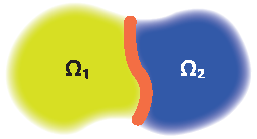
\includegraphics{chapters/chapter3/figures/blob.pdf}
\end{minipage}
\begin{minipage}{0.5\textwidth}
\begin{align*}
  E(\rOmega_{1}\cup\rOmega_2) &= E(\rOmega_1) + E(\rOmega_2) + W_{12} \qquad \\
  & \overset{?}{=}\mathcal{E}(\rOmega_1)+\mathcal{E}(\rOmega_2)
\end{align*}
\end{minipage}
\caption{
	The energy of an isolated system is the sum of the energies of its subsystems (as defined when they are isolated as well) plus the interaction among them, $W_{12}$, whose magnitude scales as the area of the interface, depicted in red. When defining the energies of individual subsystems, $\mathcal{E}$, $W_{12}$ has to be arbitrarily partitioned among them. \label{fig:energy-partition}}
\end{figure}

Let us consider a mono-atomic fluid interacting through pair potentials, $v(|\mathbf{R}_n-\mathbf{R}_m|)$, and define the atomic energies as \cite{Marcolongo2014,Ercole2016}:
\begin{equation}
  e_{\smallgamma,n}(\rGamma) =
  \frac{1}{2M_n}(\mathbf{P}_{n})^{2} + \frac{1}{2}\sum_{m\ne n}
  v(|\mathbf{R}_{n}-\mathbf{R}_{m}|)
  (1+\gamma_{nm}), \label{eq:gamma-atomic-energies}
\end{equation}
where $\gamma_{nm}=-\gamma_{mn}$ is \emph{any} antisymmetric matrix.
As the inter-atomic potential appearing in Eq.~\eqref{eq:gamma-atomic-energies} is symmetric with respect to the atomic indices, it is clear that the sum of all the atomic energies does not depend on $\gamma$, thus making any choice of $\gamma$ equally permissible. This trivial observation has deep consequences on the theory of thermal fluctuations and transport, because the value of the macroscopic energy flux, instead, depends explicitly on $\gamma$, thus making one fear that the resulting transport coefficients would depend on $\gamma$ as well. Using the same manipulations that lead from Eqs.~\eqref{eq:epsilon-classical} and \eqref{eq:atomic-energies} to Eq.~\eqref{eq:J-classical}, for any choice of the $\gamma$ matrix in Eq.~\eqref{eq:gamma-atomic-energies}, a corresponding expression for the macroscopic energy flux can be found, reading \cite{Marcolongo2014,Ercole2016}:
\begin{equation}
  \mathbf{J}_{\smallgamma}^\smallE=\mathbf{J}^\smallE+
  \frac{1}{2 \rOmega}\sum_{n,m\ne n}\gamma_{nm} \Bigl ( v_{nm} \mathbf{V}_{n} + \bigl (\mathbf{V}_{n}\cdot \nabla_{\mathbf{R}_n} v_{nm} \bigr )  (\mathbf{R}_{n}-\mathbf{R}_{m}) \Bigr ), \label{eq:gamma-classical-current}
\end{equation}
where $v_{nm}= v(|\mathbf{R}_{n} - \mathbf{R}_{m}|)$.

\begin{figure}
    \begin{center}
        \subfigure[\label{fig:argon-gauge-acf}]{\includegraphics[width=0.8\textwidth]{chapters/chapter3/figures/handbook_argon_egauge_acf.pdf}}
        \subfigure[\label{fig:argon-gauge-kappa}]{\includegraphics[width=0.8\textwidth]{chapters/chapter3/figures/handbook_argon_egauge_kappa.pdf}}
    \end{center}
	\caption{(a) Time correlation functions of the modified macroscopic energy flux of a Lennard-Jones fluid, at the conditions described in the text, as defined in Eq.~\eqref{eq:gamma-classical-current}, for different definitions of the $\gamma$ matrix (see text). The ``0'' line refers to the standard definition ($\gamma = 0$), whereas the labels ``1'' and ``2'' correspond to the two (arbitrary) definitions of $\gamma$ given in Eq.~\eqref{eq:gamma-definitions}.
    (b) Integral of the time correlation functions displayed in Fig.~\ref{fig:argon-gauge-acf}, multiplied by the prefactor appearing in the GK relation, Eq.~\eqref{eq:GK-complete}, as a function of the upper limit of integration. 
    The parameterss used are $\lambda_1=10$ and $\lambda_2=2.5$. The barely visible shaded area surrounding each line is an indication of the error bars, as estimated by standard block analysis. Units are Lennard-Jones units ($M=\sigma=\varepsilon=1$). \label{fig:argon-gauge}}
\end{figure}

\paragraph{An example from classical MD}
In order to illustrate this state of affairs, we have performed classical MD simulations for a Lennard-Jones monotaomic fluid described by the inter-atomic potential $v(R) = 4\varepsilon \left[ \left( \frac{\sigma}{R}\right)^{12} - \left(\frac{\sigma}{R} \right)^{6} \right]$ at temperature $T=1.86 \frac{\epsilon}{k_B}$ and density $\rho=0.925 \sigma^{-3}$, using cubic simulation cells containing 256 atoms in the iso-choric microcanonical ensemble, with the LAMMPS package \cite{LAMMPS1995}. 
In Fig.~\ref{fig:argon-gauge-acf} we display the resulting macroscopic energy-flux autocorrelation function corresponding to different choices of the $\gamma$ matrix in Eqs.~\eqref{eq:gamma-atomic-energies} and \eqref{eq:gamma-classical-current}. The $\Gamma$ matrices have been constructed in two different ways,
according to the (arbitrary) prescriptions:
\begin{equation}
\setbox0=\vbox{\hsize=50mm \small\noindent where the matrix
      elements of $A$ are drawn from a uniform deviate  in the
      $[0,\lambda]$ interval.}
\setbox1 \vbox{\hsize=50mm \small\noindent according to whether $I=J$,
  $I>J$, or $I<J$.}
\Gamma_{IJ}= \left \{
  \begin{alignedat}{2}
    \frac{1}{2} \left(A_{IJ}-A_{JI}\right ) & \quad\raise -.5\ht0
    \box0 && \qquad (1) \\
\\
    0, +\lambda, -\lambda & \quad\raise -0.5\ht1 \box1 && \qquad (2) \\
  \end{alignedat} \right .
\label{eq:gamma-definitions}
\end{equation}
In Fig.~\ref{fig:argon-gauge-acf} we display the resulting macroscopic energy-flux autocorrelation functions, $\langle \mathbf{J}_{\gamma}^{\smallE}(t) \cdot\mathbf{J}_{\gamma}^{\smallE}(0)\rangle$, that dramatically depend on the $\gamma$ matrices in Eqs.~\eqref{eq:gamma-atomic-energies} and \eqref{eq:gamma-classical-current}.  Notwithstanding, the integrals of all these time correlation functions tend to the same limit at large integration times, as shown in Fig.~\ref{fig:argon-gauge-kappa}.

\begin{LEtext}
The ill-definetess of the atomic energies and of the heat current was already noticed by some authors. \citet{Schelling2002} computed the thermal conductivity of Stillinger-Weber \cite{Stillinger1985} silicon and noticed that they were fairly insensitive to the particular definition used, and concluded that the fact that there is no rigorous and unique definition is not a serious impediment to using the GK method. Ten years later, \citet{Howell2012} studied the same system more extensively, and found that the energy decomposition in the three-body interaction term gives a negligible contribution to the computed thermal conductivity, even though he considered the two-body atomic energy well-defined.

How is it that different definitions of the energy flux would lead to the same value for the thermal conductivity? The fundamental origin of this conundrum involves the two main properties of the total energy: extensivity and conservation, and leads us to the discovery of a gauge invariance principle for thermal transport coefficients.
\end{LEtext}


\section{Gauge invariance}

In order to get insight into this remarkable invariance property, let us inspect the difference between the generalized flux in Eq.~\eqref{eq:gamma-classical-current} and the standard expression of Eq.~\eqref{eq:J-classical}:
\begin{equation}
  \rDelta\mathbf{J}^\smallE_{\smallgamma} =\mathbf{J}^\smallE_{\smallgamma}-\mathbf{J}^\smallE  =\frac{\mathrm{d}}{\mathrm{dt}}\frac{1}{4 \rOmega} \sum_{n,m\ne n}  \gamma_{nm} \, v(|\mathbf{R}_{n}-\mathbf{R}_{m}|)  (\mathbf{R}_{n}-\mathbf{R}_{m}). \label{eq:DeltaJ}
\end{equation}
We see that the two different expressions for the macroscopic energy flux differ by a total time derivative of a bounded phase-space vector function. In the following, we show that this is a consequence of energy conservation and extensivity and a sufficient condition for the corresponding thermal conductivities to coincide.

The very possibility of defining an energy current density, from which the energy fluxes of Eq.~\eqref{eq:J-classical} and \eqref{eq:gamma-classical-current} ultimately depend, stems from energy extensivity, \emph{i.e.} the energy of a macroscopic sample of matter of volume $\Omega$ can be written as the integral of an energy density, $e(\mathbf{r})$:
\begin{equation}
  E[\Omega]=\int_{\Omega}e(\mathbf{r})d\mathbf{r}. \label{eq:E-extensivity}
\end{equation}
Along the same considerations illustrated in Fig.~\ref{fig:energy-partition}, the energy density appearing in Eq. \eqref{eq:E-extensivity} is not uniquely defined:  any 
two densities $e'(\mathbf{r},t)$ and $e(\mathbf{r},t)$, whose integrals over a macroscopic volume differ by a quantity that scales as the volume boundary, should be considered as equivalent. 
This equivalence can be expressed by the condition that two equivalent densities differ by the divergence of a (bounded) vector field:
\begin{equation}
  e'(\mathbf{r},t)=e(\mathbf{r},t) - \nabla\cdot \bm{p}(\mathbf{r},t). \label{eq:gauge_transformation}
\end{equation}
In a sense, two equivalent energy densities can be thought of as different \emph{gauges} of the same scalar field. 

Energy is also conserved: because of this, for any given gauge of the energy density, $e(\mathbf{r},t)$, an energy current density can be defined, $\bm{j}(\mathbf{r},t)$, so as to satisfy the continuity equation, Eq.~\eqref{eq:continuity}:
\begin{equation}
  \dot{e}(\mathbf{r},t)=-\nabla\cdot
  \mathbf{j}_{e}(\mathbf{r},t). \label{eq:energy-continuity} 
\end{equation}
By combining Eqs.~\eqref{eq:gauge_transformation} and \eqref{eq:energy-continuity} we see that energy current densities and macroscopic fluxes transform under a gauge transformation as:
\begin{align}
 \bm{j}'(\mathbf{r},t) & = \bm{j}(\mathbf{r},t) + \dot{\bm{p}}(\mathbf{r},t), \label{eq:current_density_gauge} \\
  \mathbf{J}'(t) & = \mathbf{J}(t) + \dot{\mathbf{P}}(t), \label{eq:macroscopic_flux_gauge}
\end{align}
where $\mathbf{P}(t)=\frac{1}{\rOmega} \int\bm{p}(\mathbf{r},t)d\mathbf{r}$. We
conclude that the macroscopic energy fluxes in two different energy gauges differ by the total time derivative of a bounded phase-space vector function.

We now show that the energy fluxes of the same system in two different energy gauges, $e$ and $e'$, differing by a bounded total time derivative, as in Eq.~\eqref{eq:macroscopic_flux_gauge}, result in the same heat conductivity, as given by the Green-Kubo formula, Eq.~\eqref{eq:GK-complete}. More generally, the Onsager coefficients coupling two fluxes, $\mathbf{J}^1$ and $\left(\mathbf{J}^1\right)'$, do not depend on the gauge of either one of them. In fact, let $\left(\mathbf{J}^1\right)' = \mathbf{J}^1 + \dot{\mathbf{P}}$; one has:
\begin{equation}
  \begin{aligned}
    \left (L^{11} \right)' &= \frac{\rOmega}{2 k_B }\int_{-\infty}^{+\infty} \left \langle \left (\mathbf{J}^1(t)+\dot{\mathbf{P}}(t) \right ) \cdot  \left (\mathbf{J}^1(0)+\dot{\mathbf{P}}(0)\right ) \right \rangle dt \\
    &= L^{11} + \frac{\rOmega}{2 k_B } \left[ \left .  \left \langle \mathbf{P}(t) \cdot \dot{\mathbf{P}}(0) \right \rangle \right |^{+\infty}_{-\infty} + \left .  2 \Bigl \langle \mathbf{P}(t) \cdot \mathbf{J}^1(0) \Bigr \rangle \right |^{+\infty}_{-\infty} \right] ,
  \end{aligned} \label{eq:L=L'}
\end{equation}
where we used the property that classical auto-correlation functions are even in time.

The expectation of the time-lagged products in Eq.~\eqref{eq:L=L'} factorizes into the products of two independent expectations at large time lag. As the equilibrium expectations of both a total time derivative and a current vanish, we conclude that $\left (L^{11}\right )'=L^{11}$. Heat conductivities computed in different energy gauges coincide, as they must on physical grounds. A slight generalization of this argument, also using microscopic reversibility as in Ref.~\cite{Onsager1931a,Onsager1931b}, allows us to conclude that $\left (L^{12} \right )'=L^{12}$ and that, in general, $\kappa'=\kappa$.

\bigskip
\LEnote{*** INSERISCI GAUGE INVARIANCE IN FORMA DI TEOREMA ***}


\subsection{Alternative proof}
\begin{LEtext}
An alternative proof of the gauge invariance of the Onsager coefficients can be obtained using the Lemma described by \citet{Marcolongo2016}.
\begin{theorem}[Aris-Schwartz] \label{th:aris-theorem}
Let $\mathbf{J}_A$ and $\mathbf{J}_B$ be two macroscopic fluxes defined for the same system, and  $\mathbf{J}_{C} = \mathbf{J}_A + \mathbf{J}_B$ be their sum. The corresponding Onsager coefficients\footnote{For the sake of simplicity, with $L^A$ we indicate the $1-1$ component of the Onsager matrix, but it is straightforward to generalize the theorem to the other components.}, $L^{A}$, $L^{B}$, and $L^{C}$ satisfy the relation:
\begin{equation} \label{eq:aris-theorem}
    \left| L^{C} - L^{A} - L^{B} \right| \leq 2 \sqrt{L^{A} L^{B}}
\end{equation}
\end{theorem}
\begin{proof}
The Einstein-Helfand relation correspondent to the flux $\mathbf{J}^A$ states that 
\begin{equation}
    L^{X} = \lim_{\mathcal{T}\rightarrow\infty} \frac{\left\langle|\mathcal{D}^X(\mathcal{T})|^2\right\rangle} {\mathcal{T}},
\end{equation}
where $\mathcal{D}^X(\tau)=\int_0^\tau \mathbf{J}^X(\Gamma_t) dt$ is the displacement associated with the flux $\mathbf{J}^A$ (see Eq.~\eqref{eq:Einstein-Helfand-Lij}). It follows that 
\begin{equation}
    L^{C} = L^{A} + L^{B} + \lim_{\mathcal{T}\rightarrow\infty} \frac{2\left\langle \mathcal{D}^A(t) \cdot \mathcal{D}^B(t)\right\rangle} {t}.
\end{equation}
Canonical averages of products of phase-space functions can be seen as scalar products:
\footnote{Let us consider two random variables, $X$ and $Y$, and $Z=(X+aY)^2$, where $a\in \mathbb{R}$ is a constant. By definition $Z$ is not negative, and $0\leq \langle Z \rangle = \langle X^2 \rangle + a^2 \langle Y^2 \rangle + 2a \langle XY \rangle$. If we take $a = -\frac{\langle XY \rangle}{\langle Y^2 \rangle}$, we obtain the Schwartz inequality
\begin{equation} \label{eq:schwartz-ineq}
    |\langle XY \rangle| \leq \sqrt{\langle X^2 \rangle} \sqrt{\langle Y^2 \rangle}.
\end{equation}}
therefore, thanks to the Cauchy-Schwartz inequality, we have that $\lim_{\mathcal{T}\rightarrow\infty} \frac{2\left\langle \mathcal{D}^A(t) \cdot \mathcal{D}^B(t)\right\rangle} {t} \leq 2\sqrt{L^{A} L^{B}}$, that proves the theorem. 
\end{proof}

\begin{proof}[Proof (alternative)]
Alternatively, we can express the Onsager coefficients as the zero-frequency value of the correspondent power spectrum (or cross spectrum), as in Eq.~\eqref{eq:GK-S0}, \emph{i.e.} $L^{X} \propto S^{XX}(\omega=0)$. We obtain that
\begin{align}
    S^{CC}(\omega=0) &= \int_{-\infty}^\infty \langle J^C_t J^C_0 \rangle dt \nonumber\\
        &=\int_{-\infty}^\infty \left(\langle J^A_t J^A_0 \rangle + \langle J^B_t J^B_0 \rangle + 2\langle J^A_t J^B_0 \rangle \right) dt  \nonumber\\
        &= S^{AA}(\omega=0) + S^{BB}(\omega=0) + 2 S^{AB}(\omega=0),
\end{align}
where we used the fact the $\langle J^A_t J^B_0 \rangle = \langle J^B_t J^A_0 \rangle$, and from Eqs.~\eqref{eq:Sij(omega)} we have:
\begin{equation}
    S^{AB}(\omega=0) = \left\langle \frac{\int_0^\mathcal{T} J^A_t dt}{\sqrt{\mathcal{T}}} \frac{\int_0^\mathcal{T} J^B_t dt}{\sqrt{\mathcal{T}}} \right\rangle + \mathcal{O}(\mathcal{T}^{-1}) .
\end{equation}
Thanks to the Schwartz inequality, Eq.~\eqref{eq:schwartz-ineq}, we must have that
\begin{equation}
\begin{aligned}
    0 \leq \left|S^{AB}(\omega=0)\right| &\leq \sqrt{\left\langle\frac{1}{\mathcal{T}}\left(\int_0^\mathcal{T} J^A_t dt\right)^2\right\rangle} \sqrt{\left\langle\frac{1}{\mathcal{T}}\left(\int_0^\mathcal{T} J^B_t dt\right)^2\right\rangle} \\
    &= \sqrt{S^{A}(\omega=0) S^{B}(\omega=0)} .
\end{aligned}
\end{equation}
for each $\mathcal{T}>0$, from which Eq.~\eqref{eq:aris-theorem} follows.
\end{proof}
\end{LEtext}


\section{Molecular fluids}  \label{sec:MolecularFluids}
In a one-component molecular fluid such as liquid water or, say, ethanol, there are in general $Q$ fluxes interacting with each other through Onsagers' Eq.~\eqref{eq:onsager}, where $Q$ is the number of atomic species in a molecule. The requirement that atoms are bound in molecules of fixed composition, however, sets a number of constraints that substantially simplify the treatment of heat transport, making the molecular case similar to the one-component one.

Let us consider a molecule of chemical formula $A_{N_A} B_{N_B}\cdots$, where $A, B,\cdots$ indicate atomic species, and $N_A,N_B,\cdots$ the corresponding atomic stoichiometric indices. For each atomic species we define the normalized number flux as:
\begin{equation}
  \mathbf{J}^X = \frac{1}{N_X}\sum_{n\in X} \mathbf{V}_n. \label{eq:JX}
\end{equation}
If we indicate by $M_X$ the atomic mass of species $X$, momentum conservation requires that $\sum_X M_X N_X \mathbf{J}^X = 0$ in the center-of-mass reference frame. The flux $\mathbf{J}^{XY} = \mathbf{J}^{X}-\mathbf{J}^{Y}$ is the total time derivative of a bounded vector, because its integral is the sum over all the molecules of the difference between the average atomic positions of either species within a same molecule, which is obviously bounded if molecules do not dissociate. As any number flux $\mathbf{J}^X$ can be expressed as a linear combination of the total momentum and of several $\mathbf{J}^{XY}$ fluxes, each of them is the total time derivative of a bounded vector. Therefore, the Onsager coefficient coupling any of these atomic fluxes with any other, or with the energy flux, vanishes. We conclude that energy is the only conserved quantity relevant for heat transport in a molecular fluid, and that the energy-flux autocorrelation function directly yields the thermal conductivity, as in Eq.~\eqref{eq:GK}.


\section{Comment on the classical definition of heat flux in solids}  \label{sec:carbogno}

...

\section{Outlook}  \label{sec:gauge-outlook}

\begin{LEtext}
The discovery of the gauge invariance principle provides the theoretical foundation for the formulation of a theory of adiabatic heat transport within density functional theory (DFT). The first such formulation is presented in Chapter~\ref{ch:dft-heat}. 

Furthermore, this principle opens the possibility of designing the definition of the local energy (both in terms of atomic energies or energy densities), so as to optimize the convergence of the thermal conductivity estimator.
Aris-Schwartz theorem, Eq.~\eqref{eq:aris-theorem}, ensures that if a flux $\mathbf{J}_B$ does not contribute to the conductivity (\emph{i.e.} it has a vanishing GK integral, $L^B=0$), it is possible to the define a new flux $\mathbf{J}_C=\mathbf{J}_A+\mathbf{J}_B$ that will yield the same conductivity of $\mathbf{J}_A$. Even though $L^C=L^A$, the statistical properties of two such equivalent currents need not to be the same, in that the fluctuations of their correlation functions will be different, and the resulting GK integral of Eq.~\eqref{eq:GK-complete} will depend differently on the upper limit of integration, as it was the case in the example shown in Fig.~\ref{fig:argon-gauge}.
We shall see that in the particular case of DFT thermal transport, for some peculiar systems, the definition of energy density and flux may make the estimate of the thermal conductivity very difficult, due to the large statistical fluctuations of the correlation functions. In this case, the gauge invariance principle can come to the rescue.
\end{LEtext}
  % Gauge invariance
\chapter{Density-functional theory of adiabatic heat transport} \label{ch:dft-heat}

\begin{LEtext}
The advent of density-functional theory (DFT) \cite{Hohenberg1964,Kohn1965} has marked the start of a new era for the quantum modeling of materials. DFT allows computing interatomic forces entirely from first principles using the chemical composition and the fundamental laws of nature as the sole ingredients, without any need to leverage experimental knowledge of these interactions.
Its combination with classical molecular dynamics, both in the Born-Oppenheimer of Car-Parrinello flavours \cite{Car1985,Marx2009}, had a groundbreaking impact in a wide number of physical problems.

Nevertheless, quantum simulation methods based on DFT have long been thought to be incompatible with the GK theory of thermal transport \emph{because in first-principles calculations it is impossible to uniquely decompose the total energy into individual contributions from each atom} \cite{Stackhouse2010b}. For this reason, \emph{ab initio} simulations of heat transport have often been performed using non-equilibrium approaches.

The recently discovered gauge invariance principle that was introduced in Chapter~\ref{ch:gauge-invariance} not only explains why an arbitrary defintion of the heat flux results in a well-defined value for the thermal conductivity, but it also gives a rigorous way of deriving an expression for the energy flux directly from DFT, without introducing any \emph{ad hoc} ingredients.

In this chapter we first summarize the most recent \emph{ab initio} methods for the computation of thermal conductivity. Then we briefly review the first-principles GK theory of thermal transport developed by \citet{Marcolongo2014}, that will be adopted in the rest of this work.
\end{LEtext}


\section{First-principles simulation methods}
\begin{LEtext}
In insulators heat transport is determined by the dissipative dynamics of atoms, the electrons following adiabatically in their ground state, a regime often referred to as atomic or \emph{adiabatic heat conduction}. Different approaches are available to model heat conduction in these systems: the main ones are the \emph{Boltzmann's transport equation} (BTE), \emph{non-equilibrium Green's functions} (NEGF), and \emph{molecular dynamics} (MD), both in its non-equilibrium and equilibrium flavors. 

\emph{Non-equilibrium Green's functions} (NEGF) \cite{Wang2008} are designed to compute the conductance of open systems, such as nanoscale devices and interfaces, but they do not apply to bulk conduction. 

The \emph{Boltzmann's transport equation} (BTE) \cite{Peierls1929,Zhou2016} is the method of choice for crystals well below melting, where long-lived phonons are clearly identified as the heat carriers. In this case density-functional perturbation theory \cite{Baroni1987a,Gonze1989,Baroni2001} allows one to compute accurate phonon frequencies \cite{Giannozzi1991} and lifetimes, \cite{Debernardi1995,Paulatto2013} and thus implement the BTE entirely from first principles \cite{Broido:2007iu}. 
The flexibility and accuracy of \abinitio BTE are such that this approach is being successfully used to screen new materials for custom-designed properties, such as high thermal conductivity for passive cooling \cite{Lindsay:2013fw,Lindsay:2013db} or low thermal conductivity for thermoelectric energy conversion \cite{PhysRevX.4.011019,Schwingen2014}. 
Recent self-consistent and variational approaches to solve the BTE beyond the relaxation-time approximation \cite{Fugallo2013} are also providing fresh and deep insight into the collective character of heat transport \cite{Fugallo2013,Lee:2015ex,Cepellotti2015,Cepellotti:2016bk}. 
Yet, the applicability of \emph{ab initio} BTE is restricted to periodic systems consisting of a small number of atoms per unit cell, and is severely limited by its own inherent approximations: as the temperature increases, anharmonic effects become so important as to eventually make it break down well below melting \cite{Turney:2009bb}, while the BTE simply does not apply to glasses and liquids, where phonons are not even defined \cite{Allen1989} .

\emph{Molecular dynamics} (MD) \cite{Allen1989,Frenkel2001} is set to overcome these limitations. 
In non-equilibrium MD (NEMD) \cite{Evans1990,Muller-Plathe1997}, temperature gradients or heat fluxes are explicitly imposed on the virtual sample, and the thermal conductivity is estimated from the resulting value of the conjugate variable (flux or gradient). 
In the so-called \emph{approach to equilibrium} (AEMD) methodology of \citet{Lampin2013} the system is first prepared in an out-of-equilibrium state, characterized by an inhomogeneous temperature distribution, and the thermal conductivity is evaluated from the time it takes for the system to equilibrate. 
NEMD and AEMD lend themselves to a straightforward quantum-mechanical implementation \cite{Stackhouse2010b,Bouzid2017} using \emph{ab initio} molecular dynamics (AIMD). For example, \citet{Stackhouse2010b} computed the thermal conductivity of periclase MgO using a method devised by \citet{Muller-Plathe1997}, \emph{i.e.} by imposing a temperature gradient to the system, and evaluating the ratio between the heat flux and the resulting temperature gradient.
\citet{Bouzid2017} combined AEMD with AIMD to simulate thermal transport in a GeTe$_4$ glass, while \citet{Puligheddu2017} further generalized and applied it to crystalline and nano-structured MgO.
However, but methods may be both affected by non-linear effects, due to the strength of the temperature gradient to be imposed \cite{Schelling2002,He2012} and by finite-size/finite-time effects that require long simulation times and difficult extrapolations to approach the thermodynamic limit \cite{sellan2010,He2011,He2012,Zaoui2016,Wang2017}. 

The combination of equilibrium molecular dynamics (EMD), based on the Green-Kubo theory, with DFT, has been successfully accomplished very recently by \cite{Marcolongo2016}, thanks to the gauge-invariance principle introduced in Chapter~\ref{ch:gauge-invariance}, that gives a rigorous way of deriving an expression for the energy flux directly from DFT, without introducing any \emph{ad hoc} ingredients. We describe this approach in Sec.~\ref{sec:dft-heat-theory} and we will use it in the rest of this work. (***RIFERIMENTI***)

More recently, several works attempted to combine the GK approach to heat transport with first-principles techniques based on electronic-structure theory, by adopting some \emph{ad hoc} definitions for the energy flux. \citet{Kang2017}, for instance, derived an expression for the energy flux from a (rather arbitrary) quantum-mechanical definition of the atomic energies and used a modified MD integration algorithm to cope with the difficulties ensuing from the implementation of their expression in PBC. 
\citet{Carbogno:2017gc} gave a different expression for the energy flux, that neglects the convective term (**EQ.**) and is based on a normal-mode decomposition of the atomic coordinates and forces, which, while allowing to reduce the effects of thermal fluctuations, can only be applied to crystalline solids.

\citet{English2017}, instead, used the classical Einstein relation for the energy displacement, $\mathcal{D}(\tau) = \sum_n \mathbf{R}_n \int_0^\tau \mathbf{F}_n \cdot \mathbf{V}_n \, dt$, computed from a BO-AIMD trajectory, where the forces are computed from the Hellmann-Feynman theorem. They applied this methodology to the computation of thermal conductivity of periclase MgO \cite{Tse2018} and other solids. Their approach also neglects the convective term and is only applicable to solids.
\end{LEtext}


\section{DFT energy flux}  \label{sec:dft-heat-theory}
The gauge invariance principle presented in Chapter~\ref{ch:gauge-invariance} provides a rigorous way to derive an expression for the adiabatic energy flux from DFT.
In order to derive such an expression, we start with the standard DFT expression of the total energy in terms of the Kohn-Sham (KS) eigenvalues $\varepsilon_v$, eigenfunctions $\phi_v(\mathbf{r})$, and density $n(\mathbf{r}) = \sum_v |\phi_v(\mathbf{r})|^2$ \cite{Martin2008}:\footnote{For simplicity, here and in the following we imply the dependence on time $t$ of atomic positions, velocities and KS orbitals.}
\begin{multline}
  E_{\smallDFT} = \frac{1}{2}\sum_{n}M_{n}V_{n}^{2} + \frac{\mathtt{e}^2}{2}\sum_{n,m\ne n}\frac{ Z_{n}Z_{m}}{|\mathbf{R}_{n}-\mathbf{R}_{m}|} \\
  + \sum_{v}\varepsilon_{v}-\frac{\mathtt{e}^2}{2}\int\frac{n(\mathbf{r})n(\mathbf{r}')}{|\mathbf{r}-\mathbf{r}'|}d\mathbf{r}d\mathbf{r}'+\int\left(\epsilon_{\smallXC}[n](\mathbf{r})-\mu_{\smallXC}[n](\mathbf{r})\right)n(\mathbf{r})d\mathbf{r},
\end{multline}
where $\{\mathbf{R}\}$ and $\{\mathbf{r}\}$ indicate ionic and electronic positions, respectively, $\mathtt{e}$ is the electron charge, $\epsilon_\smallXC[n](\mathbf{r})$ is a local exchange-correlation (XC) energy per particle defined by the relation $ \int \epsilon_\smallXC[n](\mathbf{r})n(\mathbf{r}) d\mathbf{r}=E_\smallXC [n]$, the latter being the total XC energy of the system, and $ \mu_\smallXC (\mathbf{r}) = \frac{\delta E_\smallXC }{\delta n(\mathbf{r})}$ is the XC potential. The DFT total energy can be readily written as the integral of a DFT energy density (not uniquely defined) \cite{Chetty1992}:
\begin{align}
    E_{\smallDFT} & =  \int e_{\smallDFT}(\mathbf{r})d\mathbf{r}, \nonumber\\
    e_{\smallDFT}(\mathbf{r}) & = e_{el}(\mathbf{r})+e_{\smallZ}(\mathbf{r}), \label{eq:DFT-Edensity}
\end{align}
where:
\begin{align}
  e_{el}(\mathbf{r}) & =\mathfrak{Re} \sum_{v}\phi_{v}^{*}(\mathbf{r})\bigl(H_{\smallKS}\phi_{n}(\mathbf{r})\bigr) \nonumber \\
  & \qquad\qquad\qquad - \frac{1}{2}n(\mathbf{r})v_{\smallH}(\mathbf{r}) +\left(\epsilon_\smallXC (\mathbf{r}) - \mu_\smallXC  (\mathbf{r}) \right) n(\mathbf{r}), \\
  e_{\smallZ}(\mathbf{r}) & = \sum_{n}\delta(\mathbf{r}-\mathbf{R}_{n}) \left(\frac{1}{2}M_{n}V_{n}^{2}+w_{n}\right), \\
  w_{n} & =\frac{\mathtt{e}^2}{2}\sum_{m\ne n}\frac{ Z_{n}Z_{m}}{|\mathbf{R}_{n}-\mathbf{R}_{m}|}, \label{eq:DFT-Edensity-breakup}
\end{align}
$H_\smallKS$ is the instantaneous self-consistent Kohn-Sham Hamiltonian, and $v_\smallH = \mathtt{e}^2 \int d\mathbf{r}' \frac{n(\mathbf{r}')}{|\mathbf{r}-\mathbf{r}'|}$ is the Hartree potential. 

An explicit expression for the DFT energy flux is obtained by computing the first moment of the time derivative of the energy density, Eqs.~(\ref{eq:DFT-Edensity}-\ref{eq:DFT-Edensity-breakup}), as indicated in Eq.~\eqref{eq:JE=rdote}, 
\begin{equation}
    \mathbf{J}^\smallE = \frac{1}{\rOmega} \int \dot e_{\smallDFT}(\mathbf{r}) \,\mathbf{r}\, d\mathbf{r} ,
\end{equation}
and considering the Born-Oppenheimer (BO) equations of motion for the nuclei:
\begin{equation}
    M_n \dot{\mathbf{V}}_n = -\frac{\partial E_{\smallDFT}}{\partial \mathbf{R}_n} .
\end{equation}
This results in a number of terms, some of which are either infinite or ill-defined in PBC. Casting the result in a regular, boundary-insensitive, expression requires a careful breakup and refactoring of the various harmful terms \cite{Marcolongo2014,Marcolongo2016}. The final result reads:
\begin{align}
  \allowdisplaybreaks
  \mathbf{J}^\smallE_{\smallDFT}  &=  \mathbf{J}^{\smallH} + \mathbf{J}^{\smallZ} + \mathbf{J}^{0} + \mathbf{J}^{\smallKS} +  \mathbf{J}^{\smallXC}, \label{eq:DFT-Eflux}\\
  \mathbf{J}^{\smallH}  &=  \frac{1}{4\pi \rOmega \mathtt{e}^2}\int \nabla v_{\smallH}(\mathbf r) \dot v_{\smallH}(\mathbf  r) d\mathbf{r}, \\
  \mathbf{J}^{\smallZ}  &=  \frac{1}{\rOmega} \sum_{n}  \left[\mathbf{V}_{n}\left(\frac{1}{2}M_{n}V_{n}^{2} + w_{n}\right) + \sum_{m\ne n}(\mathbf{R}_{n} - \mathbf{R}_{m}) \left(\mathbf{V}_{m} \cdot \frac {\partial w_{n}}{\partial \mathbf{R}_{m}} \right) \right], \label{eq:DFT-ionic}\\
  \mathbf{J}^{0}  &=  \frac{1}{\rOmega}  \sum_{n} \sum_{v}\left\langle \phi_{v} \middle| (\mathbf{r}-\mathbf{R}_{n})\left(\mathbf{V}_{n}\cdot\frac{\partial\hat{v}_{0}}{\partial\mathbf{R}_{n}}\right)\middle| \phi_{v}\right\rangle, \\
  \mathbf{J}^{\smallKS}  &=  \frac{1}{\rOmega} \sum_{v} \left( \langle \phi_v | \mathbf{r} H_{\smallKS} | \dot\phi_v \rangle + \varepsilon_v \langle \phi_v | \mathbf{r} | \dot\phi_v \rangle \right)  =  \frac{1}{\rOmega}  \mathfrak{Re} \sum_{v} \left\langle \bm{\bar \phi}_v^c \middle| H_{\smallKS}+\varepsilon_v \middle| \dot \phi_v^c \right\rangle, \label{eq:DFT-KS}\\
  J_\alpha^{\smallXC}  &=
    \begin{cases}
        0 & \mathrm{(LDA)} \\
        -\frac{1}{\rOmega} \int n(\mathbf{r}) \dot{n}(\mathbf{r}) \frac{\partial\epsilon^{\smallGGA} (\mathbf{r})}{\partial(\partial_\alpha n)} d\mathbf{r} & \mathrm{(GGA)},
    \end{cases}
\end{align}
where  $\hat v_0$ is the bare, possibly non-local, (pseudo-) potential acting on the electrons and
\begin{align}
  |\bm{\bar \phi}_v^c\rangle &= \hat P_c \,\mathbf{r}  \,|\phi_v \rangle, \label{eq:r-times-phi} \\
  |\dot \phi_v^c\rangle &= \hat P_c |\dot\phi_v\rangle = \dot{\hat P}_v \,|\phi_v\rangle, \label{eq:phi-dot}
\end{align}
are the projections over the empty-state manifold of the action of the position operator over the $v$-th occupied orbital, Eq.~\eqref{eq:r-times-phi}, and of its adiabatic time derivative \cite{Giannozzi2017}, Eq.~ \eqref{eq:phi-dot}; $\hat P_v$ and $\hat P_c = 1 - \hat P_v$ being the projector operators over the occupied- and empty-states manifolds, respectively. Both these functions are well defined in PBC and can be computed, explicitly or implicitly, using standard density-functional perturbation theory \cite{Baroni2001}.


\subsection{Electronic current}
\begin{LEtext}
The current $\mathbf{J}^\smallKS$, Eq.\eqref{eq:DFT-KS}, is not manifestly invariant with rspect to the arbitrary choice of the zero of the one-electron energy levels: a shift of this zero by a quantity $\Delta\epsilon$ results in a shift of the energy flux by $\Delta \mathbf{J}^{el}$, where $\mathbf{J}^{el}$ is the adiabatic electronic current \cite{Thouless1983},
\begin{equation}
 \mathbf J^{el} = \frac{2}{\rOmega}\mathfrak{Re} \sum_{v} \langle\bm{\bar \phi}_v^c |\dot \phi_v^c \rangle, \label{eq:DFT-electronic}
\end{equation}
that can be derived from the continuity equation for the electronic density:
\begin{equation}
\nabla\cdot \bm j^{el}(\bm r,t) =- \dot{n}^{el}(\bm r,t).    
\end{equation}
The electronic current is the difference between the total charge current and its ionic component. In insulators the first is by definition non-diffusive, while the second vanishes in the center of mass of mono-atomic and molecular systems, because of momentum conservation (see Sec.~\ref{sec:multi-component}). Therefore, the electronic flux $\mathbf{J}^{el}$ is non-diffusive in insulators, \emph{i.e.} it does not contribute to the thermal conductivity, lifting the apparent indeterminacy of Eq.~\eqref{eq:DFT-electronic}.
\end{LEtext}


\subsection{Multi-component heat flux}
\LEnote{*********}


\subsection{Numerical computation}
The computation of the DFT energy flux, Eq.~\eqref{eq:DFT-ionic}, at time $t$ requires the atomic positions $\{\mathbf{R}\}$ and velocities $\{\mathbf{R}\}$, along with the Kohn-Sham eigenvalues $\varepsilon_v$, eigenfunctions $\phi_v(\mathbf{r})$, the ground-state electron density distributions $n(\mathbf{r}) = \sum_v |\phi_v(\mathbf{r})|^2$ and their time-derivatives. 

The calculation is performed within the \textsc{Quantum Espresso} code suite \cite{Giannozzi2009,Giannozzi2017} in a specialized post-processing code (not yet publicly available). In order to compute the energy flux $\mathbf{J}^\smallE$, one should first extract a sufficient number of time steps from a AIMD trajectory (the sampling frequency should be high enough to avoid aliasing problems: a deeper discussion on this is reported in Sec.~***REF-SAMPLING*****). For each of these time steps, two self-consistent KS calculations are performed with the \textsc{PWscf} code: one at time $t$ and one at time $t+\Delta t$. The resulting densities are used to compute the time derivative of the electron density at time $t$, $\dot{n}(t)$, with finite differences: $\dot{n}(t) = (n(t+\Delta t) - n(t))/\Delta t$.
Therefore, the cost of one energy flux calculation is about equal to the cost of two self-consistent calculations plus one linear response calculation. *******
In the current implementation, each time step costs almost 4 times the cost of a self-consistent calculation.
The atomic coordinates at time $t+\Delta t$ are extrapolated from those at time $t$, simply as $\mathbf{R}(t+\Delta t) = \mathbf{R}(t) + \mathbf{V}(t) \Delta t$. The value of the finite difference $\Delta t$ is very important, and is much smaller than the time step used to evolve the dynamics with MD. A convergence check should be performed beforehand, as shown in Fig.~***** for the case of liquid water.******

\bigskip
\LEnote{*******FIGURA CONVERGENZA TIMESTEP*********}

\bigskip
\LEnote{***** ESEMPI ARIS?? ***}


\section{Outlook}  \label{sec:dft-outlook}
As it was already mentioned in Sec.~\ref{sec:gauge-outlook}, the gauge invariance of transport coefficients not only provides a solid foundation to the quantum theory of adiabatic heat transport, by also allows tuning this definition so as to achieve optimal statistical properties to reduce its computational cost. This freedom can in principle be exploited to design new expressions for the heat flux. One possibility may be devising a formulation base on a local representation of the electronic structure \cite{Marzari2012,Damle2015}, \emph{e.g.} maximally localized Wannier functions, that would avoid the use of density-functional perturbation theory for the computation of $\mathbf{J}^{\smallKS}$, by removing the ill-definiteness problems in PBC. In the case of solids, where correlation times are generally longer, a more efficient expression may be obtained from a normal-mode expansion \cite{Ladd1986} and interpolation, to cope with noise and finite-size effects, in a similar way to the one proposed by \citet{Carbogno:2017gc}. 

Furthermore, the expression of the energy flux, that is now implemented for LDA and GGA energy functionals, can be extended to more advanced functionals \cite{French_2010:long_range,Berland2015}, where dispersion forces are accounted for. This effects are important in the structural and transport properties of many soft materials.

Finally, the \abinitio computation of thermal conductivity of multi-component fluids has never been attempted and would be particularly beneficial to study systems in extreme conditions.  % DFT heat transport
\chapter{Data analysis}  \label{ch:data-analysis}

The MD evaluation of the GK integral, Eq.~\eqref{eq:GK}, usually proceeds in two steps. One first evaluates the integrand as a running average of the time-lagged current products, $\langle J^i(\tau)J^j(0)\rangle \sim \frac{1}{\mathcal{T}-\tau} \int_0^{\mathcal{T}-\tau} J^i(t+\tau)J^j(t)dt$, where $\mathcal{T}$ is the length of the MD trajectory.
The matrix defined in Eq.~\eqref{eq:L_def} is then estimated as a function of the upper limit of integration:  $L^{ij}(\mathcal{T})\propto \frac{\rOmega}{k_B} \int_0^\mathcal{T} \langle J^i(\tau)J^j(0)\rangle \,d\tau$. One then recovers, via Eq.~\eqref{eq:multi_kappa}, an estimate for the thermal conductivity depending on $\mathcal{T}$:
$\kappa(\mathcal{T})\propto \frac{1}{(L^{-1}(\mathcal{T}))^{\smallone\smallone}}$.
This function is usually very noisy: in fact, at times greater than the correlation time between $J^i$ and $J^j$, the correlation function $\langle J^i(\tau)J^j(0)\rangle$ approaches zero, hence $L^{ij}(\mathcal{T})$ starts integrating noise and behaves like the distance traveled by a random walk, whose variance grows linearly with the upper integration limit.
The evaluation of transport coefficients thus requires averaging over multiple trajectories (possibly multiple segments of a same long trajectory) and estimating the resulting uncertainty as a function of both the length of each trajectory and the upper limit of integration. This is a cumbersome task that often leads to a poor estimate of the statistical and systematic errors on the computed conductivity. All the more so when the signal is inherently oscillatory, due to the existence of high-frequency features in the power spectrum of the energy flux, possibly due to intramolecular oscillations that meddle with the noise. Some authors try to overcome these problems by either fitting the autocorrelation function or the GK integral with a multi-exponential function \citep{Schelling2002,Zhang2015}, or by extrapolating the power spectrum of the energy flux to the zero-frequency limit \citep{Volz2000}. Others have attempted an error analysis of the MD estimate of the GK integral, based on either heuristic or rigorous arguments \citep{Jones2012,Wang_gk2017,Oliveira2017}, but they all require an estimate of an optimal value for the upper limit of integration, which determines a bias in the estimate, and which is in general difficult to obtain. Different classes of systems require different approaches to error analysis, but it is widely believed that all of them always require so long simulation times as to be unaffordable with accurate but expensive AIMD techniques \citep{Carbogno:2017gc}. In order to solve this problem, \cite{Ercole2017} considered it in the light of the statistical theory of stationary time series.


\section{Solids and one-component fluids} \label{sec:univariate}
In practice, MD gives access to a discrete sample of the flux process (a \emph{time series}), $J_n = J(n \epsilon)$, $0 \leq n \leq N-1$, where $\epsilon$ is the sampling period of the flux and $N$ the length of the time series, that we assume to be even. As was shown in Sec.~\ref{sec:Einstein}, the Wiener-Khintchine theorem allows one to express the heat conductivity in terms of the zero-frequency value of the power spectrum of the energy-flux (see Eqs.~(\ref{eq:Wiener-Khintchine}-\ref{eq:GK-S0})):
\begin{equation}
\kappa = \frac{\rOmega}{2k_B T^2} S (\omega=0). \label{eq:kappa-S0}
\end{equation}
Let us define the discrete Fourier transform of the flux time series as:
\begin{equation}
  \tilde{J}_{k}=\sum_{n=0}^{N-1} \mathrm{e}^{ 2\pi i\frac{kn}{N}} J_n, \label{eq:Jk}
\end{equation}
for $0 \leq k \leq N-1$.\footnote{Here, the convention for the sign in the exponential of the time-to-frequency Fourier transform is opposite to what adopted in \citep{Ercole2017} and in most of the signal analysis literature, in order to comply with the convention for the space-time Fourier transforms usually adopted in the Physics literature and in Eqs.~\eqref{eq:kontinuity} and \eqref{eq:Fourier-continuity}.} The \emph{sample spectrum} $\hat S_k$, aka \emph{periodogram}, is defined as
\begin{equation}
\hat{S}_{k}=\frac{\epsilon}{N} \left |\tilde{J}_{k} \right |^2, \label{eq:periodogram-def}
\end{equation}
and, for large $N$, it is an unbiased estimator of the power spectrum of the process, as defined in Eq.~\eqref{eq:Wiener-Khintchine}, evaluated at $\omega_k=2\pi\frac{k}{N\epsilon}$, namely: $\langle \hat S_k \rangle = S(\omega_k)$. The reality of the $\hat J$'s implies that $\tilde J_k=\tilde J^*_{N-k}$ and $\hat S_k=\hat S_{N-k}$, so that periodograms are usually reported for $0\leq k\leq \frac{N}{2}$ and their Fourier transforms evaluated as discrete cosine transforms.

The space autocorrelations of conserved currents are usually short-ranged. Therefore, in the thermodynamic limit the corresponding fluxes can be seen as sums of (almost) independent identically distributed stochastic variables, so that, according to the central-limit theorem, their equilibrium distribution is Gaussian. A slight generalization of this argument allows us to conclude that any conserved-flux process is Gaussian as well. The flux time series is in fact a multivariate stochastic variable that, in the thermodynamic limit, results from the sum of (almost) independent variables, thus tending to a multivariate normal deviate. This implies that at equilibrium the real and imaginary parts of the $\tilde J_k$'s defined in Eqs.~\eqref{eq:Jk} are zero-mean normal deviates that, in the large-$N$ limit, are uncorrelated among themselves and have variances proportional to the power spectrum evaluated at $\omega_k$. For $k=0$ or $k=\frac{N}{2}$, $\tilde J_k$ is real and $\sim \mathcal{N}\left (0, \frac{N}{\epsilon}S(\omega_k) \right )$; for $k\notin\left\{ 0,\frac{N}{2}\right\}$, $\mathfrak{Re}\tilde{J}_k$ and $\mathfrak{Im}\tilde{J}_k$ are independent and both  $\sim \mathcal{N}\left (0, \frac{N}{2 \epsilon}S(\omega_k) \right )$, where $\mathcal{N} (\mu,\sigma^2)$ indicates a normal deviate with mean $\mu$ and variance $\sigma^2$. We conclude that in the large-$N$ limit the sample spectrum of the heat-flux time series reads:
\begin{equation}
\hat{S}_{k} = S \left(\omega_k\right) {\xi}_{k}, \label{eq:periodogram-distribution}
\end{equation}
where the $ {\xi}$'s are independent random variables distributed as a $\chi_1^2$ variate for $k=0$ or $k=\frac{N}{2}$ and as one half a $\chi_2^2$ variate, otherwise. Here and in the following $\chi^2_\nu$ indicates the chi-square distribution with $\nu$ degrees of freedom. For the sake of simplicity, we make as though all the ${\xi}$'s were identically distributed, $\xi_k \sim \frac{1}{2} \chi_2^2$ for all values of $k$, thus making an error of order $\mathcal{O}(1/N)$, which vanishes in the long-time limit that is being assumed throughout this section.

In many cases of practical interest, multiple time series are available to estimate the power spectrum of a same process, $\{{^p\!}J_n\}$, $p=1, \cdots \ell$. For instance, in equilibrium MD a same trajectory delivers one independent time series per Cartesian component of the heat flux, all of which are obviously equivalent in isotropic systems. In these cases it is expedient to define a mean sample spectrum by averaging over the $\ell$ different realizations,
\begin{equation}
    \begin{aligned}
      {^{\ell\!}\hat{S}}_{k}& = \frac{\epsilon}{\ell N} \sum_{p=1}^{\ell}  \left |{^p\!}{\tilde J}_{k} \right |^2 \\
      & = S \left(\omega_k\right) {^{\ell\!}{\xi}_{k}},
    \end{aligned} \label{eq:mean-periodogram}
\end{equation}
where the ${^{\ell\!}\xi}$'s are $\chi_{2\ell}^2$ variates, divided by the number of degrees of freedom: $^{\ell\!}\xi_{k}\sim\frac{1}{2\ell}\chi_{2\ell}^{2}$ $\bigl (\text{for } k \notin \{ 0,\frac{N}{2} \}\bigr )$.

\begin{figure}
\centering
\includegraphics[width=8cm]{chapters/chapter5/figures/handbook_water_psd.pdf}
\caption{Periodogram of a classical flexible model of water obtained from a $100\un{ps}$ MD trajectory. Grey: periodogram obtained directly from Eq.~\eqref{eq:mean-periodogram}, with $\ell=3$. Blue: periodogram filtered with a moving average window of width $1\un{THz}$, useful to reveal the main features of the spectrum (see text). The vertical dashed line delimits the low-frequency region used in the subsequent cepstral analysis.}  \label{fig:water-periodogram}
\end{figure}

Eqs.~\eqref{eq:periodogram-distribution}) and \eqref{eq:mean-periodogram} show that ${^{\ell\!}}{\hat S_0}$ is an unbiased estimator of the zero-frequency value of the power spectrum, $\langle {^{\ell\!}}{\hat S_0} \rangle = S(0)$, and through Eq.~\eqref{eq:kappa-S0}, of the transport coefficients we are after. However, this estimator is not consistent, \emph{i.e.} its variance does not vanish in the large-$N$ limit. This is so because a longer time series increases the number of discrete frequencies at which the power spectrum is sampled, rather than its accuracy at any one of them.

Fig.~\ref{fig:water-periodogram} displays the periodogram of water at ambient conditions, obtained from a $100\un{ps}$ classical MD trajectory, showing the extremely noisy behavior of the periodogram as an estimator of the spectrum. Averaging over the values of the periodogram within a frequency window of given width \citep{MovingAverage} would consistently reduce the statistical noise, but the multiplicative nature of the latter in Eq.~\eqref{eq:periodogram-distribution} makes it difficult to disentangle the noise from the signal and may introduce a bias. In order to cope with this problem, we had better transform the multiplicative noise into an additive one by defining the log-periodogram, $^{{\ell\!}}\hat{L}_{k}$, as:
\begin{equation}
  \begin{aligned}
    ^{{\ell\!}}\hat{L}_{k} &= \log \left (^{\ell\!}\hat{S}_{k} \right ) \\
    &= \log\left(S(\omega_k) \right) + \log\left( ^{\ell\!}{\xi}_k\right ) \\
    &= \log\left(S(\omega_k) \right) + {^{\ell\!}\rLambda} + {^{\ell\!}{\lambda}}_{k},
  \end{aligned} \label{eq:log-PSD}
\end{equation}
where $^{\ell\!}{\lambda}_k = \log\left( {^{\ell\!}{\xi}}_k\right) - {^\ell{\rLambda}}$
are zero-mean identically distributed independent stochastic variables, ${^{\ell\!}\rLambda} = \left\langle \log\left( {^{\ell\!}{\xi}}\right ) \right\rangle = \psi(\ell)-\log(\ell)$, and $\psi(z)$ and is the digamma function \citep{PolyGamma}. The variance of the $^{\ell\!}\lambda$ variables is $\sigma_{\ell}^{2} =\psi'(\ell)$, where $\psi'(z)$ is the tri-gamma function \citep{PolyGamma}.

Whenever the number of (inverse) Fourier components of the logarithm of the power spectrum is much smaller than the length of the time series, applying a low-pass filter to Eq.~\eqref{eq:log-PSD} would result in a reduction of the power of the noise, without affecting the signal. In order to exploit this idea, we define the ``\emph{cepstrum}'' of the time series as the inverse Fourier transform of its sample log-spectrum \citep{Childers1977}:
\begin{equation}
  ^{\ell\!} \hat C_{n} = \frac{1}{N}\sum_{k=0}^{N-1} {^{\ell\!} \hat L_{k}} \mathrm{e}^{-2\pi i\frac{kn}{N}}. \label{eq:sample-cepstrum}
\end{equation}
A generalized central-limit theorem for Fourier transforms of stationary time series ensures that, in the large-$N$ limit, these coefficients are a set of independent (almost) identically distributed zero-mean normal deviates \citep{Anderson1994,Peligrad2010}. It follows that:
\begin{equation}
  \begin{aligned}
    ^{\ell\!} \hat  C_{n} &= \lambda_{\ell} \delta_{n0} + C_{n} +  {^{{\ell\!}}{\mu}}_{n}, \\
    C_{n} &= \frac{1}{N}\sum_{k=0}^{N-1} \log\bigl (S(\omega_k) \bigr ) \mathrm{e}^{-2\pi i\frac{kn}{N}},
  \end{aligned} \label{eq:cepstrogram}
\end{equation}
where $^{{\ell\!}}{\mu}_{n}$ are independent zero-mean \emph{normal} deviates with variances $\left\langle {^{{\ell\!}}{\mu}_{n}^2}  \right\rangle$ $=\frac{1}{N}\sigma_\ell$ for $n\notin\left\{ 0,\frac{N}{2}\right\}$ and $\left\langle ^{{\ell\!}}{\mu}_{n}^{2}\right\rangle =\frac{2}{N}\sigma_{\ell}^{2}$
otherwise.
Fig.~\ref{fig:water-cepstrum} displays the cepstral coefficients of the low-frequency region of the spectrum of water (marked in Fig.~\ref{fig:water-periodogram}), showing that only the first few coefficients are substantially different from zero.

\begin{figure}
\centering
\includegraphics[width=8cm]{chapters/chapter5/figures/handbook_water_cepstrum.pdf}
\caption{Cepstral coefficients of water computed analyzing the low-frequency region of the periodogram (see Fig.~\ref{fig:water-periodogram}), defined in Eq.~\eqref{eq:sample-cepstrum}. }  \label{fig:water-cepstrum}
\end{figure}

Let us indicate by $P^*$ the smallest integer such that $C_n \approx 0$ for $P^* \le n \le N-P^*$. By limiting the Fourier transform of the sample cepstrum, Eq.~\eqref{eq:sample-cepstrum}, to $P^*$ coefficients, we obtain an efficient estimator of the zero-frequency component of the log-spectrum as:
\begin{equation}
  \begin{aligned}
    ^{{\ell\!}}\hat{L}_{0}^{*} & = {^{\ell\!}\hat{C}}_{0}+2\sum_{n=1}^{P^{*}-1}{^{{\ell\!}}\hat{C}}_{n} \\
    & = {^{\ell\!}\rLambda} + \log(S_0) + {^{{\ell\!}} {\mu}_{0}}+ 2 \sum_{n=1}^{P^*-1} {^{\ell\!} {\mu}_{n}}.
  \end{aligned} \label{eq:L0*}
\end{equation}
Inspection of Eq.~\eqref{eq:L0*} shows that $^{\ell\!}\hat{L}_{0}^{*}$ is a normal estimator whose expectation and variance are:
\begin{align}
	\langle {^{{\ell\!}}\hat{L}_{0}^{*}}\rangle &= \log(S_{0}) + {^{\ell\!}\rLambda}, \label{eq:L*} \\
	\sigma_\ell^{*}(P^{*},N)^{2} &=\sigma_{\ell}^{2}\frac{4P^{*}-2}{N}. \label{eq:sigma*}
\end{align}
Using Eq.~\eqref{eq:kappa-S0}, we see that the logarithm of the conductivity can be estimated from the cepstral coefficients of the flux time series through Eqs.~(\ref{eq:L0*}-\ref{eq:sigma*}), and that the resulting estimator is always normal with a variance that depends on the specifc system \emph{only} through the number of these coefficients, $P^*$. Notice that the absolute error on the logarithm of the conductivity directly and nicely yields the relative error on the conductivity itself.

The efficacy of this approach obviously depends on our ability to estimate the number of coefficients necessary to keep the bias introduced by the truncation to a value smaller than the statistical error, while maintaining the magnitude of the latter at a prescribed acceptable level. \cite{Ercole2017} proposed to estimate $P^*$ using the Akaike's information criterion (\cite{Akaike1974}), but other more advanced \emph{model selection} approaches \citep{Claeskens2008} may be more effective. This method consists in choosing $P^*$ as the one that minimizes the function:
\begin{equation}
\mathrm{AIC}(P)=\frac{N}{\sigma_\ell^{2}}\sum_{n=P}^\frac{N}{2} \hat{C}_{n}^{2}+2P. \label{eq:AIC-P}
\end{equation}
In Fig.~\ref{fig:water-filtered-psd} we report the low-frequency region of the spectrum of water obtained by limiting the number of cepstral coefficients to $P^*$:
\begin{equation}
^\ell\hat{S}_k^* = \exp\left[ 2\sum_{n=1}^{P^*-1} {}^\ell\hat{C}_n \mathrm{e}^{2\pi i \frac{k n}{N}} + {}^\ell\hat{C}_0 - {}^\ell\rLambda\right], \label{eq:filtered-psd}
\end{equation}
thus showing the filtering effect of this choice.
Finally, Fig.~\ref{fig:water-fkappa-Pstar} shows the value of thermal conductivity of water obtained through Eqs.~(\ref{eq:L0*}-\ref{eq:sigma*}).

\begin{figure}
    \centering
    \begin{center}
        \subfigure[\label{fig:water-filtered-psd}]{\includegraphics[width=8cm]{chapters/chapter5/figures/handbook_water_filtered_psd.pdf}}
        \subfigure[\label{fig:water-fkappa-Pstar}]{\includegraphics[width=8cm]{chapters/chapter5/figures/handbook_water_kappa_Pstar.pdf}}
    \end{center}
    \caption{
    (a) Filtered low-frequency region of the power spectrum of water obtained by limiting the number of cepstral coefficients to various values of $P^*$, Eq.~\eqref{eq:filtered-psd}. $P^*=7$ is the cutoff value suggested by the Akaike's information criterion, Eq.~\eqref{eq:AIC-P}. Grey: the unfiltered periodogram obtained from Eq.~\eqref{eq:periodogram-def}.
    (b) Thermal conductivity of water estimated from Eqs.~(\ref{eq:L0*}-\ref{eq:sigma*}) as a function of the cutoff, $P^*$. The colored bands indicate one standard deviation as estimated from theory. The vertical dashed line indicates the value suggested by the Akaike's information criterion, Eq.~\eqref{eq:AIC-P}.
    }
\end{figure}


\section{Multi-component fluids}
In Sec.~\ref{sec:multi-component} we have seen that in a fluid made of $Q$ atomic species there are in general $Q$ macroscopic fluxes interacting with each other through Onsager's phenomenological equations, Eq.~\eqref{eq:onsager}, not counting the different Cartesian components that do not interact amongst themselves because of space isotropy. A MD simulation thus samples $Q$ stochastic processes, one for each interacting flux, that we suppose to be stationary. These processes can be thought of as different components of a same multivariate process \citep{Bertossa2018}. As in Sec.~\ref{sec:univariate}, for the sake of generality we suppose to have $\ell$ independent samples of such a process, described by a multivariate time series of length $N$: $\{ ^{p\!}{J}^i_n \}$; $p=1,\dots \ell$; $i=1,\dots Q$; $n=0,\dots N-1$. Stationarity implies that $\langle {J}^i_n\rangle $ does not depend on $n$ and that $\langle {J}^i_n {J}^j_m \rangle$ only depends on $n-m$. We will further assume that $\langle {J}^i_n\rangle =0 $ and that $\langle {J}^i_n {J}^j_0 \rangle$ is an even function of $n$, which is the case when ${J}^i$ and ${J}^j$ have the same signature under time-reversal. By combining Eq.~\eqref{eq:multi_kappa} with Eq.~\eqref{eq:GK-S0}, we see that in order to evaluate the thermal conductivity in the multi-component case we need an efficient estimator for $\left ( S^{-1}_0\right )^{11}$, where $S^{kl}_0=S^{kl}(\omega=0)$ is the zero-frequency cross-spectrum of the relevant fluxes, ordered in  such a way that the energy one is the first.

Similarly to the one-component case, we define a mean sample cross-spectrum (or \emph{cross-periodogram}) as
\begin{equation}
 ^{(\ell Q)\!}\hat{S}_k^{ij} = \frac{1}{\ell} \sum_{p=1}^{\ell} \frac{\epsilon}{N} \left({}^{p\!}\tilde{J}_k^i\right)^* {}^{p\!}\tilde{J}_k^j .
\end{equation}
By discretizing Eq.~\eqref{eq:Sij(omega)} we see that $^{(\ell Q)\!}\hat{S}_k^{ij}$ is an unbiased estimator of the cross-spectrum, $\left \langle {}^{(\ell Q)\!}\hat{S}_k^{ij} \right \rangle = S^{ij}\left (\omega_k= \frac{2\pi k }{N\epsilon}\right )$. As it was the case for univariate processes, in the large-$N$ limit the real and imaginary parts of $\tilde J^i_k$ are normal deviates that are uncorrelated for $k\ne k'$. We conclude that the cross-periodogram is a random matrix distributed as a complex Wishart deviate \citep{Goodman1963a,Goodman1963b}:
\begin{equation}
  {}^{(\ell Q)\!}\hat{S}_k \sim \mathcal{CW}_Q \left(S(\omega_k), \ell\right). \label{eq:ComplexWishart}
\end{equation}
The notation $\mathcal{CW}_Q \left(S, \ell \right)$ in Eq.~\eqref{eq:ComplexWishart} indicates the distribution of the $Q\times Q$ Hermitian matrix
${}^{(\ell Q)\!}\hat{S}^{ij} = \frac{1}{\ell}\sum_{p=1}^\ell  {}^{p\!}{X}^i \, {}^{p\!}{X}^{j*}$,
where $\{ {}^{p\!}{X}^i \}$ ($p=1,\cdots\ell$, $i=1, \cdots Q$) are $\ell$ samples of an $Q$-dimensional zero-mean normal variate whose covariance is $S^{ij} = \langle X^i X^{j*} \rangle $.

Similarly to the real case, a Bartlett decomposition \citep{kshirsagar1959} holds for complex Wishart matrices \citep{Nagar2011}, reading:
\begin{equation}
{}^{(\ell Q)\!}\hat{S} = \frac{1}{\ell} \mathcal{S} R R^\top \mathcal{S}^{\dagger},  \label{eq:S_cholesky}
\end{equation}
where ``$\top$'' and ``$\dagger$'' indicate the transpose and the adjoint of a real and complex matrix, respectively; $\mathcal{S}$ is the Cholesky factor of the covariance matrix, $S= \mathcal{S} \mathcal{S}^{\dagger}$, and $R$ is a real lower triangular random matrix of the form
\begin{equation}
 R =
 \begin{pmatrix}
 c_1 & 0 & 0 & \cdots & 0\\
 n_{21} &  c_2 &0 & \cdots& 0 \\
 n_{31} &  n_{32} &  c_3 & \cdots & 0\\
\vdots & \vdots & \vdots &\ddots & \vdots \\
 n_{\smallQ1} & n_{\smallQ2} & n_{\smallQ3} &\cdots & c_\smallQ
 \end{pmatrix},
\end{equation}
where $c^2_i \sim \chi^2_{2(\ell-i+1)}$ and $ n_{ij}\sim \mathcal{N}(0,1)$. We stress that $R$ is independent of the specific covariance matrix, and only depends upon $\ell$ and $Q$. In particular it is independent of the ordering of the fluxes $J^i$. By expressing the $QQ$ matrix element of the inverse of $^{(\ell Q)}\hat{S}$ in Eq.~\eqref{eq:S_cholesky} as the ratio between the corresponding minor and the full determinant, and using some obvious properties of the determinants and of triangular matrices, we find that:
\begin{equation}
\frac{\ell}{\left({}^{(\ell Q)}\hat{S}_k^{-1}\right)^{\smallQ\smallQ}} = \frac{1}{\left(S_k^{-1}\right)^{\smallQ\smallQ}} c^2_\smallQ, \label{eq:S-1_choleskied}
\end{equation}
As the ordering of the fluxes is arbitrary, a similar relation holds for all the diagonal elements of the inverse of the cross-periodogram. We conclude that the generalization of Eq.~\eqref{eq:mean-periodogram} for the multi-component case is:
\begin{equation}
   ^{\ell}\hat{\underline{S}}_{\,k}\equiv\frac{\ell}{2(\ell-Q+1)}\frac{1}{\left( {}^{(\ell Q)}\hat{S}_k^{-1} \right)^{\smallone\smallone}} = \frac{1}{\left(S_k^{-1}\right)^{\smallone\smallone}} \, \xi_k, \label{eq:mean-multi-periodogram}
\end{equation}
where $\xi_k$ are independent random (with respect to $k$) random variables, distributed as
\begin{equation}
  \xi_k \sim
  \begin{cases}
    \frac{1}{\ell-Q+1} \,\chi^2_{\ell-Q+1}  \qquad & \mathrm{for} \; k \in \{0 , \frac{N}{2}\}, \\
 \\
 \frac{1}{2(\ell-Q+1)} \, \chi^2_{2(\ell-Q+1)} \qquad & \mathrm{otherwise}.
\end{cases}
\end{equation}
Starting from here we can apply the cepstral analysis as in the one-component case. The only difference is the number of degrees of freedom of the $\chi^2$ distribution, that becomes $2(\ell -Q+1)$, and a different factor in front of the result. Fig.~\ref{fig:grappa-periodogram} shows an example of multi-component power spectrum for a solution of water and ethanol.

\begin{figure}
\centering
\includegraphics[width=8cm]{chapters/chapter5/figures/psd_water_ethanol_40.pdf}
\caption{Multi-component power spectrum, as defined in Eq.~\eqref{eq:mean-multi-periodogram}, for a classical flexible model of a solution of water and ethanol $50\un{mol}\%$, obtained from a $100\un{ps}$ trajectory. Grey: $^{\ell}\hat{\underline{S}}_{\,k}$ obtained directly from Eq.~\eqref{eq:mean-multi-periodogram}, with $\ell=3$ and $Q=2$. Blue: $^{\ell}\hat{\underline{S}}_{\,k}$ filtered with a moving average window of width $1\un{THz}$ in order to reveal its main features. The vertical dashed line delimits the low-frequency region used in the subsequent cepstral analysis. Reproduced from \cite{Bertossa2018}.}  \label{fig:grappa-periodogram}
\end{figure}

\begin{figure}
    \begin{center}
        \subfigure[]{\includegraphics[width=8cm]{chapters/chapter5/figures/gk-grappa_capitolo_40.pdf}}
        \subfigure[]{\includegraphics[width=8cm]{chapters/chapter5/figures/convergence_water_ethanol_40.pdf}}
    \end{center}
	\caption{Convergence of the multi-component thermal conductivity estimator $\kappa$ using the direct time-integration approach and the cepstral method, for a classical flexible model of a solution of water and ethanol $50\un{mol}\%$, obtained from a $100\un{ps}$ trajectory.
(a) Direct time-integration approach in its Green-Kubo (green, as obtained from the matrix $L^{ij}(\mathcal{T})\propto\int_0^\mathcal{T} \left\langle J^i(t) J^j(0) \right\rangle dt $) and Einstein-Helfand (orange -- obtained from the  matrix $\left (L^{ij}\right )'(\mathcal{T}) \propto  \int_0^\mathcal{T}\left(1-\frac{t}{\mathcal{T}}\right) \left \langle J^i(t) J^j(0) \right \rangle dt$) formulations. The horizontal purple band indicates the value obtained by the cepstral method.
(b) Estimate of $\kappa$ with the cepstral method as a function of the number of cepstral coefficients, $P^*$, see Eqs.~(\ref{eq:L0*}-\ref{eq:sigma*}). The dashed vertical line indicates the value of $P^*$ selected by the AIC, Eq.~\eqref{eq:AIC-P}. Reproduced from \cite{Bertossa2018}.
}  \label{fig:twoCompConvergence}
\end{figure}

The method discussed so far shows a fundamental advantage with respect to a na\"ive implementation of direct time-integration approach.
Fig.~\ref{fig:twoCompConvergence} shows the two-component conductivity $\kappa$, obtained via Eq.~\eqref{eq:two-comp-kappa}, in the case of a water-ethanol solution, as a function of the upper time-integration limit $\mathcal{T}$ \citep{Bertossa2018}. Both the Green-Kubo and the Einstein-Helfand definitions of the finite-time expression of Onsager's coefficients (see Eq.~\eqref{eq:Einstein-Helfand}) are displayed.
Due to thermal fluctuations, the integral of the correlation function becomes a random walk as soon as the latter vanishes, eventually assuming any value. Therefore, there will be a set of times (see Fig.~\ref{fig:twoCompConvergence}) where the term $L^{\smallQ\smallQ}$ at the denominator in Eq.~\eqref{eq:two-comp-kappa} vanishes, leading to divergences in the evaluation of $\kappa$; an issue not affecting the one-component case. Hence, in such a formulation of the multi-component case, the mean value of the thermal conductivity estimator \textit{in the time domain} does not exist. On the contrary, the multi-component frequency-domain approach presented in this section, and built on sound statistical basis, provides a well defined expression for the estimator of $\kappa$ and its statistical error.


\section{Data analysis work-flow}
We summarize the steps leading to the estimation of thermal conductivity by the \textit{cepstral analysis} method, in order to highlight the simplicity of its practical implementation.
\begin{enumerate}
\item From a MD simulation compute the heat flux time series $J_n^1$ and the independent particle fluxes $J_n^q$, $q=2,\dots,Q$.
\item Compute the discrete Fourier transform of the fluxes, $\tilde{J}^{\small i}_k$, and the element $1/(\hat{S}^{-1})^{\smallone\smallone}$. In practice, only a selected low-frequency region shall be used (see \cite{Ercole2017} for a detailed discussion).\footnote{To lighten the notation, we drop the left superscripts of the variables in this subsection.}
\item Calculate $\log\left[1/(\hat{S}^{-1})^{\smallone\smallone}\right]$.
\item Compute the inverse discrete Fourier transform of the result to obtain the cepstral coefficients $\hat{C}_n$.
\item Apply the Akaike Information Criterion, Eq.~\eqref{eq:AIC-P}, to estimate the number of cepstral coefficients to retain, $P^*$.
\item Finally apply Eq.~\eqref{eq:L0*} to obtain $\hat{L}_0^*$, and evaluate the thermal conductivity as
\begin{equation}
\kappa = \frac{\rOmega}{2k_B T^2} \exp\left[\hat{L}_0^* - \psi(\ell - Q+1) + \log(\ell -Q+1) \right],
\end{equation}
and its statistical error as
\begin{equation}
\frac{\rDelta\kappa}{\kappa} = \sqrt{\psi'(\ell -Q+1) \frac{4P^{*}-2}{N}}.
\end{equation}
\end{enumerate}
  % Data analysis
\chapter{Thermal conductivity simulations of Silica glass}

\LEnote{*** INTRODUCTION, STATO DELL'ARTE ***}

\paragraph{Thermal conductivity of glasses}
Thermal conductivity of glass systems is a fundamental property for many industrial and technological applications, \emph{e.g.} heat management in electronic devices, windows for green architectures.
However, ``thermal conductivity represents largely explored territories, ripe for new research efforts'' [J.Mauro...]\cite{MauroFM14,Mauro2014}. The understanding of thermal conductivity and its structural origin in glasses has been greatly overlooked in the literature. 

\paragraph{Vitreous silica}
Vitreous silica has been the subject of significant research efforts in the last decades, due to is many technological applications that range from thermal insulation to laser engineering, semiconductor fabrication, and optical communication.
In particular, thanks to its excellent UV transparency, mechanical stability, and chemical durability, silica can be used in many optical applications, such as the diffractive elements and the protective windows of the optics assemblies of inertial confinement fusion facilities. In these facilities, extremely intense nanosecond laser pulses are used and seriously challenge the durability the optical glasses. It is indeed well established that the small defects or impurities of the glass may induce damage craters due to local lattice heating and melting, that will result in a rapid optical degradation \cite{Miller2004,Canaud2004,Miller2010,Chambonneau2014,Kuzuu1999,Stuart1995,Wong2006,Carr2010,Saito2000}. The interpretation of this damage process requires the study of thermal transport and the prediction of the thermal conductivity. 

Furthermore, amorphous silica serves as the basis of multicomponent silica glasses, that are adopted for a wide range of special applications. 
Therefore predicting the thermal conductivity of silica is the first step to predict the thermal conductivity of more complicated glasses, whose elements are characterized by a complex chemistry that is difficult to model.

**Esempio vetri borosilicati ecc**

\LEnote{**AEROGELS: \small Silica aerogel, a highly porous material first synthesized in the
early thirties [1], are currently being produced using a sol–gel process
such as hydrolyzing tetramethoxysilane (TMOS) to form silica and
methanol, and subsequently dried through supercritical drying together
with carbon dioxide [2]. Silica aerogel has several highly desirable
properties including being environmentally safe, having high optical
transmission as well as large thermal resistance [3]. These properties
make silica aerogel very suited for applications such as thermal and
acoustic insulation in buildings and appliances, passive solar energy
collection devices, and dielectrics for integrated circuits [4]. Also, it is a
suitable substitute for chlorofluorocarbon-based plastics in thermal
insulation of refrigerators. The most well-known application was in
Cherenkov radiators [5] as Cherenkov counters. Another crucial characteristic
of aerogels is their extremely low density for a solid, which can
go as low as 0.003 g/cm3
. Comparatively, the density of air is approximately
0.0012 g/cm3
, which is only three times lower than that of the
silica aerogel. This would represent significant weight savings when
used in various monolithic structures. **}

%%%%%%%%%%%%%%%%%%%%%%%%%%%%%%%%%%%%%%%%%%%%%
\section{Classical simulations: sample}

\subsection{Force field}

A cooling rate of $5\un{K/ps}$ is commonly used in the literature and it was shown to generate reasonable glass structures.

(Vedi Lane PRE 92 12320) The density depends on the quenching rate and on the force field used.

The structure of amorphous silica is made of a continuous random network of silicon atoms tetrahedrally bonded to bridging oxygen atoms (2-fold coordinated).

BKS works suprisingly well, not only for silica polymorfs, but also for vitreous silica.

\citet{Tian2017} compared the structures of silica obtained from different force fields. They quenched a fully melted silica box of density $\rho=2.2\un{g/cm^3}$ from $5000\un{K}$ to $300\un{K}$ at $5\times 10^{12}\un{K/s}$ in the NVT ensemble. 
The BKS, Teter, and ReaxFF potentials all generate realistic silica structures \cite{Vollmayr1996,Yu2016,Yuan2001}, with radial distribution functions, neutron structure factors, and coordination numbers that reasonably reproduce the experimental observations.
The radial distribution functions present a first sharp peak at $\sim 1.6\un{\angstrom}$ that corresponds to the Si-O bond length, a second peak at $\sim 2.6\un{\angstrom}$ that represents the distance between two O atoms
The coordination numbers can be used to detect coordination defects, by choosing a cutoff length for Si-O pairs of $\sim 2.0\un{\angstrom}$: BKS and Teter potentials reproduce a realistic coordination environment for Si and O, with over $99.6\%$ of atoms being normally coordinated (4-fold Si and 2-fold O). \LE{**Realistic silica samples present a ***\% of cordination defects}. ReaxFF, instead, tends to generate more coordination defects, with $\sim 97.5\%$ of normally coordinated atoms.
\LEnote{**tenere discorsi coordinazione??**}

Of course the quenching rate largely influences the number of defects of the generated glass. 
\LE{**discussed in sezione dopo**}

\paragraph{Thermal conductivity}
Many studies of the thermal conductivity of a-SiO$_2$ are based on NEMD simulations, that are strongly size dependent and require the study of its convergence at large cell sizes.

With the BKS potential, at $T=300\un{K}$, $\rho=2.2\un{g/cm^3}$, \citet{Tian2017} obtained a value of thermal conductivity of $\kappa\approx 2.27\un{W/mK}$ at the maximum size simulated, whereas \citet{Coquil2011} obtained $\kappa\approx 2.10\un{W/mK}$. 

Using the relation.... extrapolation

For the Teter and ReaxFF potential, \citet{Tian2017} extracted a value of $2.5\un{W/mK}$ and $1.28\un{W/mK}$, respectively. Therefore the ReaxFF potential seems to best reproduce the experimental result of $\kappa_{exp}\approx 1.3\un{W/mK}$.


\citet{McGaughey2004b} used the GK method to estimate the thermal conductivity of a system of $576$ atoms (\LE{$\rho=***$}), obtaining a thermal conductivity of $1.96\un{W/mK}$. 
The GK method is much less affected by finite size effets, and much smaller systems can be used to simulate the bulk \cite{Schelling2002}, much smaller than the estimated mean-free path of phonons. As already mentioned in Sec.~\ref{sec:spectral-methods}, the finite size effects of the GK method may be attributed to memory effects, \emph{i.e.} to phonons that reenter the simulation box several times without scattering, thanks to PBC, and that may introduce artificial correlations. In this case, the heat flux autocorrelation function may not be realiable for times longer than the time required for the passage of the phonon across the simulation cell. 

\paragraph{VDOS}
Besides the structure of the generated sample, which is quite similar for different force fields like the BKS, Teter, and ReaxFF, what determine the thermal conductivity of the system are its vibrational properties, that can be ... with vibrational density of states.


BKS
\begin{figure}
    \centering
    \includegraphics[]{chapters/chapter6/figures/BKSW.pdf}
    \caption{BKS potential with Wolf truncation.}
    \label{fig:BKS-potential}
\end{figure}

\subsection{Sample preparation}


\subsection{Quenching}

%%%%%%%%%%%%%%%%%%%%%%%%%%%%%%%%%%%%%%%%%%%%%
\section{Classical simulations: thermal conductivity}

\subsection{Cepstral analysis}
\paragraph{Dependence on cutoff frequency $f^*$}
(For the chosen sample at experimental density)
(comparison bw normal and vel-renormalized results)

\begin{figure}
    \centering
    \subfigure[\label{fig:csilica-sample-expdens-fstar-100ps}]{\includegraphics[width=8cm]{chapters/chapter6/figures/silica_expdens_kappa_fstar_VR_100ps.pdf}}
    \subfigure[\label{fig:csilica-sample-expdens-fstar-1ns}]{\includegraphics[width=8cm]{chapters/chapter6/figures/silica_expdens_kappa_fstar_VR_1ns.pdf}}
    \subfigure[\label{fig:csilica-sample-expdens-fstar-10ns}]{\includegraphics[width=8cm]{chapters/chapter6/figures/silica_expdens_kappa_fstar_VR_10ns.pdf}}
    \caption{Dependence of $\kappa$ on the choice of the cutoff frequency $f^*$, estimated from \emph{one} sample of (a) $100\un{ps}$, (b) $1\un{ns}$, and (c) $10\un{ps}$ of the ``original'' and VR heat flux time series. 
    The original and VR periodograms are reported for reference with grey and black lines, respectively.}
    \label{fig:csilica-sample-expdens-fstar}
\end{figure}
Fig.~\ref{fig:csilica-sample-expdens-fstar} -- stability of $\kappa$ as a function of $f^*$ increases with the length of the trajectory, as its predicted error decreases. The values and errors of $\kappa$ obtained from the VR time series are equivalent to the ones obtained from the original time series, and are slightly more stable with $f^*$. This is probably due to the much smaller power of the power spectrum of the VR heat flux, that may decrease the small artifacts introduced by the low-pass filter applied before resampling. 
Any frequency in the central region of the spectrum can be taken as $f^*$, hence we choose to set $f^*=28\un{THz}$. Conversely, a $f^*$ too small makes $\kappa$ deviate sensibly, due to the fact that the low-pass filter is not strong enough to avoid aliasing effects that modify the spectrum of the resampled time series; instead, a $f^*$ that is too high ($f^*\gtrsim 60\un{THz}$) induces a bias in $\kappa$, due to the fact the log-periodogram diverges to negative values and we start to have problems of numerical precision.

  % Silica
\thischaptertocfalse
\chapter{Conclusions}  \label{ch:conclusions}

\begin{itemize}
    \item GK for complex real systems, interfaces, ...
\end{itemize}  % Conclusions

\appendix

\chapter{Classical definitions of energy flux in solids}  \label{ch:appendix-carbogno}

In this appendix we demonstrate the equivalence between two formulations of the classical energy current in solids, Eqs.~\eqref{eq:J-classical} and \eqref{eq:J-leyla}, by using the gauge invariance principle presented in Sec.~\ref{sec:gauge-invariance}. 

Let us consider the general formula of the energy flux for classical force fields, Eq.~\eqref{eq:J-classical}, and rewrite it in the following way:
\begin{align}
    \mathbf{J}_A^\smallE (\rGamma) &= \frac{1}{\Omega} \sum_n \left( \mathbf{J}_c^\smallE + \mathbf{J}_v^\smallE \right) \nonumber\\
        &= \frac{1}{\Omega} \sum_n \left( \dot{\mathbf{R}}_n \epsilon_n + \mathbf{R}_n \dot{\epsilon}_n \right) , \label{eq:apx-J-classical}
\end{align}
where $\mathbf{J}_c^\smallE$ and $\mathbf{J}_v^\smallE$ are the ``convective'' and ``virial'' components of the energy flux, as defined in Eqs.~(\ref{eq:J-convective}-\ref{eq:J-virial}). 
In solids, the definition of Eq.~\eqref{eq:J-leyla} can be adopted, that can be rewritten as:
\begin{equation}
    \mathbf{J}_B^\smallE(\rGamma) =
       \frac{1}{\rOmega} \sum_{n,m} \mathbf{R}_n^0 \dot{\epsilon}_n , \label{eq:apx-J-leyla}
\end{equation}
where $\mathbf{R}_n = \mathbf{R}_n^0 + \mathbf{u}_n$, $\mathbf{R}_n^0$ denotes the average atomic position of atom $n$, and $\mathbf{u}_n$ its instantaneous displacement. 
According to the gauge invariance theorem (p.~\pageref{th:gauge-invariance}), in order to ensure that $\mathbf{J}_B^\smallE(\rGamma)$ is equivalent to $\mathbf{J}_A^\smallE(\rGamma)$, that is it yields the same thermal conductivity, we just need to prove that their difference is \emph{non-diffusive}, \emph{i.e.} it is a total time derivative of a bounded vector. 
After a few manipulations we have:
\begin{align}
    \mathbf{J}_A^\smallE(\rGamma) - \mathbf{J}_B^\smallE(\rGamma) 
        &= \frac{1}{\Omega} \sum_n \left( \dot{\mathbf{R}}_n \epsilon_n + \mathbf{R}_n \dot{\epsilon}_n - \mathbf{R}_n^0 \dot{\epsilon}_n \right) \nonumber\\
        &= \frac{1}{\Omega} \sum_n \left( \dot{\mathbf{u}}_n \epsilon_n + \mathbf{u}_n \dot{\epsilon}_n \right) \nonumber\\
        &= \frac{1}{\Omega} \frac{d}{dt} \sum_n \dot{\mathbf{u}}_n \epsilon_n ,
\end{align}
where we used the fact that $\dot{\mathbf{R}}_n = \dot{\mathbf{u}}_n$.
The sum $\sum_n \dot{\mathbf{u}}_n \epsilon_n$ is a function of the phase-space that is well-defined in PBC, and it is a bounded quantity, in a solid where atomic diffusion does not occur. Therefore we can conclude that $\mathbf{J}_B^\smallE(\rGamma)$ and $\mathbf{J}_A^\smallE(\rGamma)$ result in the same thermal conductivity. 

The same cannot be concluded for the sole ``virial'' term $\mathbf{J}_v^\smallE$, for which we have that:
\begin{align}
    \mathbf{J}_A^\smallE(\rGamma) - \mathbf{J}_v^\smallE(\rGamma) 
        &= \frac{1}{\Omega} \sum_n \dot{\mathbf{R}}_n \epsilon_n  \nonumber\\
        &= \frac{1}{\Omega} \sum_n \dot{\mathbf{u}}_n \epsilon_n  \nonumber\\
        &= \mathbf{J}_A^\smallE(\rGamma) - \mathbf{J}_B^\smallE(\rGamma) - \frac{1}{\Omega} \sum_n \mathbf{u}_n \dot{\epsilon}_n .
\end{align}
The last two lines are not manifestly expressible as a total time derivative of a bounded vector, therefore the ``convective'' term $\mathbf{J}_c^\smallE$ cannot be neglected \emph{a priori} in a solid. The magnitude of its contribution (and that of the cross-correlations $\langle\mathbf{J}_c^\smallE(t)\cdot \mathbf{J}_v^\smallE(0)\rangle$) should be verified on a case-by-case basis, as commented in Sec.~\ref{sec:flux-classical}.


%%%%%%%%%%%%%%%%%%%%%%%%%%%%%%%%%%%%%%%%%%%%%%%%%%%%%%%%%%%%%%%%%%%%%
\chapter{Silica -- NPT quench results}  \label{ch:appendix-npt-results}

\vspace{-1cm}
\begin{figure}[!htb]
    \centering
    \includegraphics[width=\textwidth]{chapters/appendix/figures/Silica_NPT_kappa_NATconv_tesi.pdf}
    \caption{Thermal conductivity of a-SiO$_2$ at $500\un{K}$ obtained by a quench in the NPT ensemble at zero-pressure and with cooling rate $\gamma$. 
    The abscissa indicate the number of atoms of the system, each panel corresponds to a different quenching rate $\gamma$ (the relative quenching time $t_\mathrm{quench}$ is indicated in brackets). 
    The same symbols as Fig.~\ref{fig:results-class-kappa-vs-size} are used.
    }
    \label{fig:appendix-silica-class-npt-kappa-vs-size}
\end{figure}

\begin{figure}[!htb]
    \centering
    \includegraphics[width=\textwidth]{chapters/appendix/figures/Silica_NPT_kappa_NATconv_tesi.pdf}
    \caption{Thermal conductivity of a-SiO$_2$ at $500\un{K}$ obtained by a quench in the NPT ensemble at zero-pressure and with cooling rate $\gamma$. 
    Each panel corresponds to a different system size with $N_{at}$ atoms.
    The same symbols as Fig.~\ref{fig:results-class-kappa-vs-quench} are used.
    }
    \label{fig:appendix-silica-class-npt-kappa-vs-quench}
\end{figure}

\begin{figure}[!htb]
    \centering
    \includegraphics[width=12cm]{chapters/appendix/figures/dens_NPT_quench.pdf}
    \caption{Average density of a sample of $N_\mathrm{at}$ atoms at $500\un{K}$, obtained from a quench in the NPT ensemble at zero-pressure as a function of the quenching rate. The black line indicates the experimental value $\rho=2.202\un{g/cm^3}$. }
    \label{fig:appendix-silica-class-npt-density-vs-quench}
\end{figure}   % Appendix

%\bibliographystyle{unsrtnat}
%\bibliography{bibliography}
\printbibliography %[heading=bibintoc]

\end{document}